% \documentclass[russian,american]{homework}
\documentclass[2020/08/28 v2]{../../../coursework}
\setotherlanguages{russian}

\title{Games, Schooling, and Surveillance}
\subtitle{Notes on Technology in a Global Pandemic}
%\shorttitle{}
\author{Dan}{}{Leonard}
\newdate{date}{12}{05}{2020}
\date{\displaydate{date}}
\course{ANTH}{374}{Anthropology of Science and Technology}{University of Illinois at Urbana-Champaign}
\instructor{Dr}{Jenny}{}{}{Davis}

\newcommand{\mc}{\citetitle{Minecraft}}
\newcommand{\tbl}{\citetitle{Tabletop}}

\newdate{log-start}{19}{03}{2020}

\addbibresource{covid.bib}
\baseurl{https://archive.danleonard.us/scholarship/coursework/illinois/ANTH/374/covid.xhtml}

\usepackage[nolist,nohyperlinks]{acronym}
\usepackage{tikz}

\begin{document}
\maketitle
\begin{acronym}
	\acro{covid}[COVID-19]{Coronavirus Disease 2019}
	\acro{virus}[SARS-CoV-2]{severe acute respiratory syndrome coronavirus 2}
	\acro{mers}[MERS]{Middle East respiratory syndrome}
	\acro{r0}[\(R_0\)]{basic reproduction rate}
	\acro{ict}[ICT]{information communication technology}
	\acro{dp3t}[DP-3T]{decentralized privacy-preserving proximity tracing}
	\acro{IP}[IP]{Internet Protocol}
	\acro{motd}[MOTD]{message of the day}
\end{acronym}
\begin{abstract}
	\noindent The \ac{covid} crisis has caused a radical change in contemporary
	society. Whether its effects are temporary or long-lasting has yet
	to be seen; however, the use of technology during the lockdown allows
	us to study how we relate to our inventions.
	I analyze the social experience of using multiplayer video games in quarantine,
	focusing on the sandbox games \mc\ and \tbl.
	Further, the experience of video chat for collegiate education is discussed, and
	how its social milieu and power dynamic differs from that of in-person classes.
	Also discussed is the coming change to smartphone technology as a result of
	the crisis, how contact tracing technology will likely have a striking impact
	on our relations to our own personal devices as well as the class dynamic
	implicit in smartphone ownership.
\end{abstract}
\keywords{coronavirus, video games, \mc, Internet, sociolinguistics, smartphones, contact tracing}
\printkeywords

\section{Games and Interpersonal Relations}

As we collectively transition into a more reclusive lifestyle,
video games provide a sense of escapism for many, including myself.
The sychronicity afforded by online video games allows 
But what does it mean to play with others online when online is all that one
can experience? \textcite{Sicart2014} describes how one's day is
structured around the experience of play, in that \enquote{my life takes
place in the time between play}~\parencite[6]{Sicart2014}. But for those
who must now only interact through others in the form of a virtual environment,
the use of play as the bounds of social interaction serves the dual purpose of creating both play
and the daily life between.

\subsection{\mc}

\mc~\parencite{Minecraft} is a platform ripe for anthropological analysis. Its simple and relaxed
rules allow for the production of creative works in the eyes of its player.
Notably, the structure of \mc\ on the Internet is one of complete independence.
Any person, even one who does not themselves own a copy of the
game, may host server software on a home computer and expose it to the Internet
without notifying the creators of the game or any upstream authority.
In contrast with the \enquote{control} exerted by a player's requirement to
\enquote{execute an algorithm in order to win}~\parencite[35]{Galloway2004} in
single-player role-playing games, \mc\ allows for social interaction relatively
unimpeded by goals or the 
Players are thus free to create social structures and communities in virtual
space accessible only to those who know the specific \ac{IP} address of the host computer.

As described by \textcite{Ringland2016} in the context of a \mc\ server for
children with autism, these virtual spaces can be decidedly formative in
social development and in escapism from the real world.
Surveying how these communities change and adapt in a global environment of forced physical
isolation can provide insight into what it means to play. One of the more
easily-surveyable parts of a server is its \ac{motd}, the text prompt displayed
when a server is queried for its online status but before a player chooses to
connect to it. By default this is set to read \enquote{A Minecraft Server} but
is easily customizable to any string the owner desires.
As the first thing every user sees when attempting to connect, whether a new or
returning player, it serves as the initial and most basic form of
identity establishment for the server's community. How this text message
is presented thus provides a corpus of text for analysis in real-time. 

\subsubsection{On \Ac{IP} addresses and server discovery}

In the standard conception of the Internet,\footnote{IPv4, which has been technically superseded
but remains in place alongside the \(2^{128}\) addresses of IPv6.}
there are approximately four billion individual
addresses\footnote{Thirty-two binary digits (bits) are used for assignment, thus
\(2^{32} = 4,294,967,296\).}
available for assignment to connected devices. While this number appears
immense at a human scale, it is in fact fairly easy for computers to scan and
enumerate these addresses, allowing researchers to view trends on the Internet
at large. The program \citetitle{zmap}\ \parencite{zmap} can perform a scan of
the entire address space in under an hour, which was used initially to gauge
potential for this survey. However, its authors caution against its frequent use
causing excess network traffic, advising users to consult with network
administrators before deployment~\parencite{zmap-paper}.
To prevent burdening University of Illinois' network administration staff during
a critical period of escalation in remote network use, I utilized the
commercial monitoring service Shodan \parencite{Shodan} to quantify
the number of \mc\ servers online.

On \displaydate{log-start}, I initiated a program to scan the
entire Internet every half-hour for such homemade \mc\ servers.
The only data points taken were the total number of services on \ac{IP}
port 25565 using the exact phrase \enquote{Minecraft Server} and how many
of those included the word \enquote{coronavirus} in their \ac{motd}.
A plot of the data collected is shown in Fig.~\ref{fig:mcgraph}. As expected,
there is a clear increase in the number of servers referencing \ac{virus} in some way.
However, I find the total rate to be
exceptionally great. From the time I started recording, at the beginning of the
\ac{covid} crisis in the United States, there has been a near-doubling worldwide
in the total number of servers online. I see this as an unmistakable sign that
many people across the world have chosen to build online communities in direct
response to the social distancing mandated in the real world.

\begin{figure}%[hp]
	% Created by tikzDevice version 0.12.3 on 2020-05-12 15:34:07
% !TEX encoding = UTF-8 Unicode
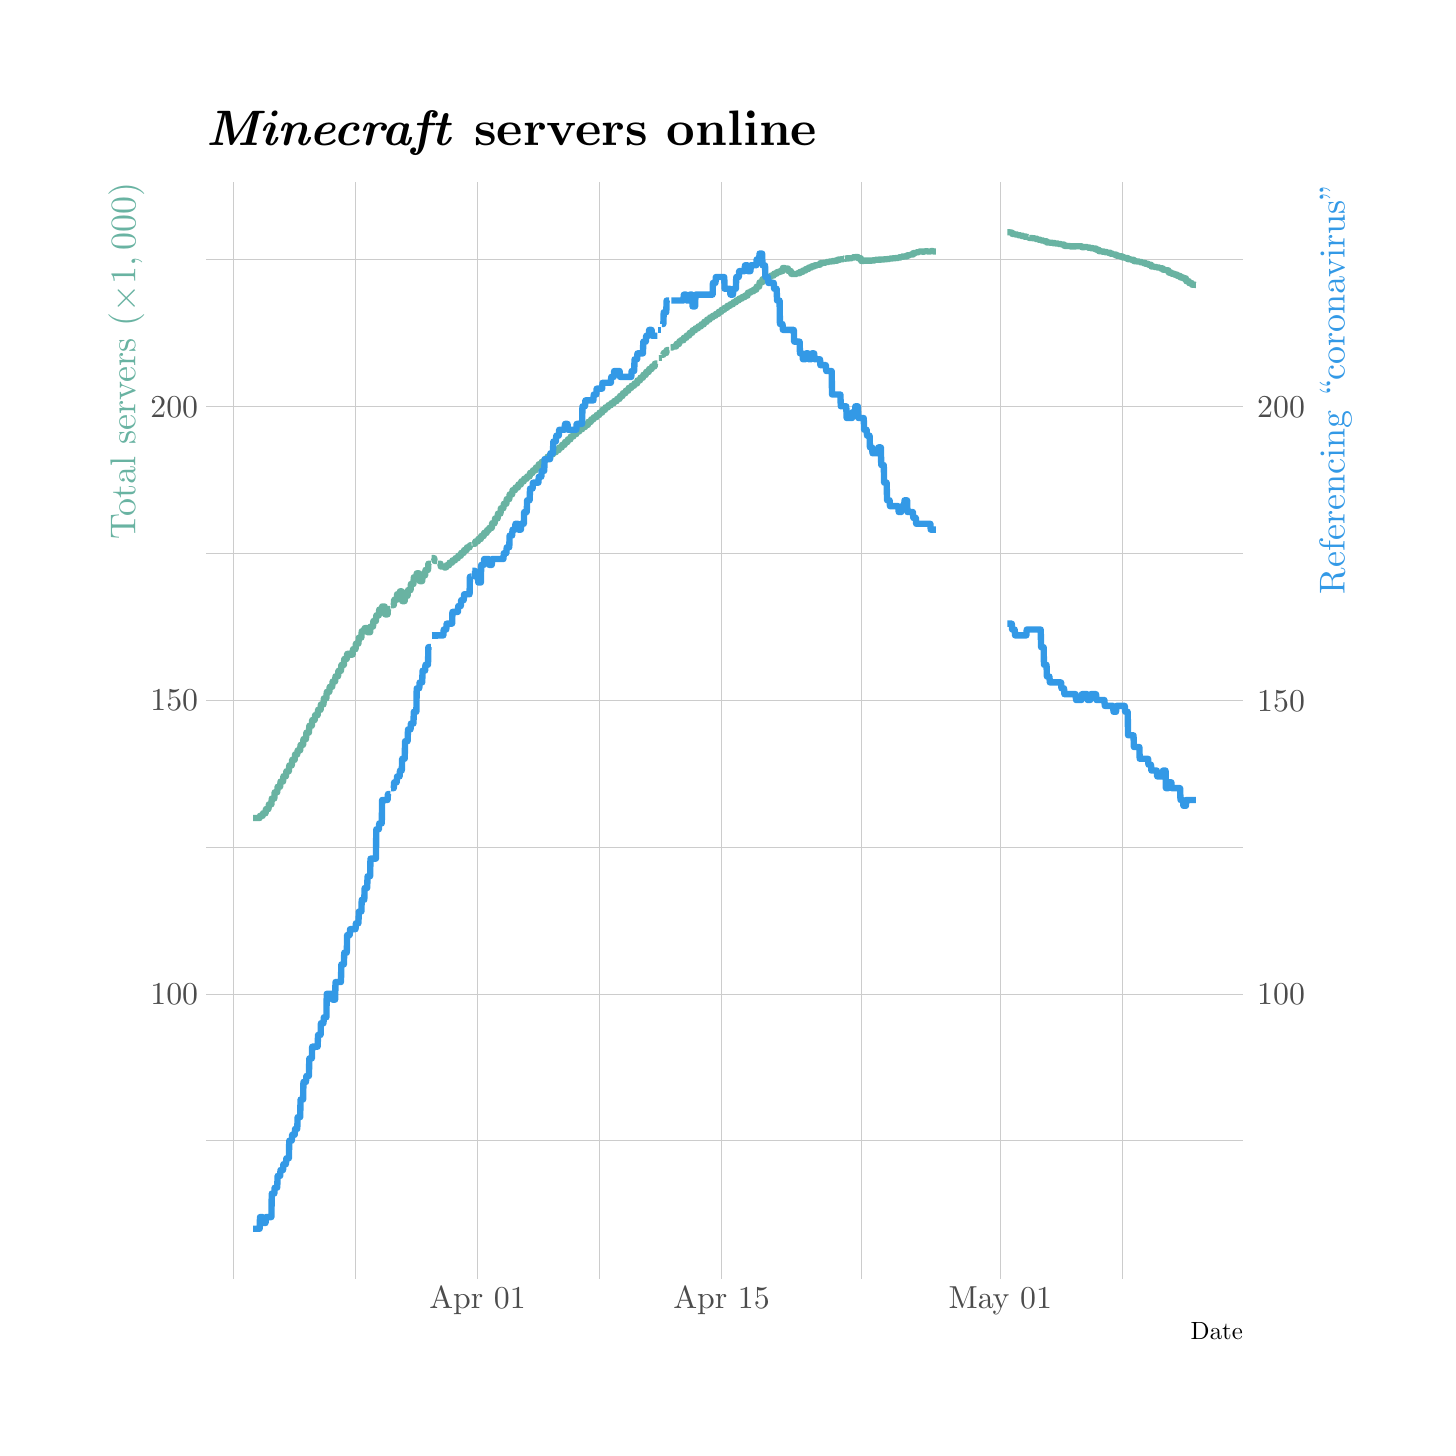
\begin{tikzpicture}[x=1pt,y=1pt]
\definecolor{fillColor}{RGB}{255,255,255}
\path[use as bounding box,fill=fillColor,fill opacity=0.00] (0,0) rectangle (505.89,505.89);
\begin{scope}
\path[clip] ( 64.48, 53.85) rectangle (439.11,449.97);
\definecolor{drawColor}{gray}{0.80}

\path[draw=drawColor,line width= 0.2pt,line join=round] ( 64.48,103.70) --
	(439.11,103.70);

\path[draw=drawColor,line width= 0.2pt,line join=round] ( 64.48,209.85) --
	(439.11,209.85);

\path[draw=drawColor,line width= 0.2pt,line join=round] ( 64.48,316.00) --
	(439.11,316.00);

\path[draw=drawColor,line width= 0.2pt,line join=round] ( 64.48,422.15) --
	(439.11,422.15);

\path[draw=drawColor,line width= 0.2pt,line join=round] ( 74.46, 53.85) --
	( 74.46,449.97);

\path[draw=drawColor,line width= 0.2pt,line join=round] (118.52, 53.85) --
	(118.52,449.97);

\path[draw=drawColor,line width= 0.2pt,line join=round] (206.65, 53.85) --
	(206.65,449.97);

\path[draw=drawColor,line width= 0.2pt,line join=round] (301.07, 53.85) --
	(301.07,449.97);

\path[draw=drawColor,line width= 0.2pt,line join=round] (395.49, 53.85) --
	(395.49,449.97);

\path[draw=drawColor,line width= 0.2pt,line join=round] ( 64.48,156.78) --
	(439.11,156.78);

\path[draw=drawColor,line width= 0.2pt,line join=round] ( 64.48,262.93) --
	(439.11,262.93);

\path[draw=drawColor,line width= 0.2pt,line join=round] ( 64.48,369.07) --
	(439.11,369.07);

\path[draw=drawColor,line width= 0.2pt,line join=round] (162.58, 53.85) --
	(162.58,449.97);

\path[draw=drawColor,line width= 0.2pt,line join=round] (250.71, 53.85) --
	(250.71,449.97);

\path[draw=drawColor,line width= 0.2pt,line join=round] (351.43, 53.85) --
	(351.43,449.97);
\definecolor{drawColor}{RGB}{105,179,162}

\path[draw=drawColor,line width= 2.3pt,line join=round] ( 81.51,220.30) --
	( 82.87,220.30) --
	( 82.90,220.30) --
	( 82.90,220.30) --
	( 83.03,220.30) --
	( 83.16,220.30) --
	( 83.29,220.30) --
	( 83.43,220.30) --
	( 83.56,220.30) --
	( 83.69,220.30) --
	( 83.82,220.30) --
	( 83.95,221.09) --
	( 83.98,221.09) --
	( 84.08,221.09) --
	( 84.25,221.09) --
	( 84.38,221.09) --
	( 84.52,221.09) --
	( 84.65,221.09) --
	( 84.78,221.09) --
	( 84.91,221.09) --
	( 85.04,222.02) --
	( 85.17,222.02) --
	( 85.31,222.02) --
	( 85.44,222.02) --
	( 85.57,222.02) --
	( 85.70,222.02) --
	( 85.83,222.02) --
	( 85.96,222.02) --
	( 86.09,223.53) --
	( 86.23,223.53) --
	( 86.36,223.53) --
	( 86.49,223.53) --
	( 86.62,223.53) --
	( 86.75,223.53) --
	( 86.88,223.53) --
	( 87.02,223.53) --
	( 87.15,225.22) --
	( 87.28,225.22) --
	( 87.41,225.22) --
	( 87.54,225.22) --
	( 87.67,225.22) --
	( 87.81,225.22) --
	( 87.94,225.22) --
	( 88.07,225.22) --
	( 88.20,227.33) --
	( 88.33,227.33) --
	( 88.46,227.33) --
	( 88.59,227.33) --
	( 88.73,227.33) --
	( 88.86,227.33) --
	( 88.99,227.33) --
	( 89.12,227.33) --
	( 89.25,229.59) --
	( 89.38,229.59) --
	( 89.52,229.59) --
	( 89.65,229.59) --
	( 89.78,229.59) --
	( 89.91,229.59) --
	( 90.04,229.59) --
	( 90.17,229.59) --
	( 90.31,231.58) --
	( 90.44,231.58) --
	( 90.57,231.58) --
	( 90.70,231.58) --
	( 90.83,231.58) --
	( 90.96,231.58) --
	( 91.10,231.58) --
	( 91.23,231.58) --
	( 91.36,233.47) --
	( 91.49,233.47) --
	( 91.62,233.47) --
	( 91.75,233.47) --
	( 91.88,233.47) --
	( 92.02,233.47) --
	( 92.15,233.47) --
	( 92.28,233.47) --
	( 92.41,235.38) --
	( 92.54,235.38) --
	( 92.67,235.38) --
	( 92.81,235.38) --
	( 92.94,235.38) --
	( 93.07,235.38) --
	( 93.20,235.38) --
	( 93.33,235.38) --
	( 93.46,237.18) --
	( 93.60,237.18) --
	( 93.73,237.18) --
	( 93.86,237.18) --
	( 93.99,237.18) --
	( 94.12,237.18) --
	( 94.25,237.18) --
	( 94.39,237.18) --
	( 94.52,239.31) --
	( 94.65,239.31) --
	( 94.78,239.31) --
	( 94.91,239.31) --
	( 95.05,239.31) --
	( 95.18,239.31) --
	( 95.31,239.31) --
	( 95.44,239.31) --
	( 95.57,241.32) --
	( 95.70,241.32) --
	( 95.83,241.32) --
	( 95.97,241.32) --
	( 96.10,241.32) --
	( 96.23,241.32) --
	( 96.36,241.32) --
	( 96.49,241.32) --
	( 96.62,243.28) --
	( 96.76,243.28) --
	( 96.89,243.28) --
	( 97.02,243.28) --
	( 97.15,243.28) --
	( 97.28,243.28) --
	( 97.41,243.28) --
	( 97.55,244.74) --
	( 97.68,244.74) --
	( 97.81,244.74) --
	( 97.94,244.74) --
	( 98.07,244.74) --
	( 98.20,244.74) --
	( 98.34,244.74) --
	( 98.47,244.74) --
	( 98.60,246.72) --
	( 98.73,246.72) --
	( 98.86,246.72) --
	( 98.99,246.72) --
	( 99.12,246.72) --
	( 99.26,246.72) --
	( 99.39,246.72) --
	( 99.52,246.72) --
	( 99.65,248.80) --
	( 99.78,248.80) --
	( 99.91,248.80) --
	(100.05,248.80) --
	(100.18,248.80) --
	(100.31,248.80) --
	(100.44,248.80) --
	(100.57,248.80) --
	(100.70,251.14) --
	(100.84,251.14) --
	(100.97,251.14) --
	(101.10,251.14) --
	(101.23,251.14) --
	(101.36,251.14) --
	(101.49,251.14) --
	(101.63,251.14) --
	(101.76,253.62) --
	(101.89,253.62) --
	(102.02,253.62) --
	(102.15,253.62) --
	(102.28,253.62) --
	(102.41,253.62) --
	(102.55,253.62) --
	(102.68,253.62) --
	(102.81,255.70) --
	(102.94,255.70) --
	(103.07,255.70) --
	(103.20,255.70) --
	(103.34,255.70) --
	(103.47,255.70) --
	(103.60,255.70) --
	(103.73,255.70) --
	(103.86,257.47) --
	(103.99,257.47) --
	(104.13,257.47) --
	(104.26,257.47) --
	(104.39,257.47) --
	(104.52,257.47) --
	(104.65,257.47) --
	(104.78,257.47) --
	(104.92,259.39) --
	(105.05,259.39) --
	(105.18,259.39) --
	(105.31,259.39) --
	(105.44,259.39) --
	(105.57,259.39) --
	(105.71,259.39) --
	(105.84,259.39) --
	(105.97,261.34) --
	(106.10,261.34) --
	(106.23,261.34) --
	(106.36,261.34) --
	(106.50,261.34) --
	(106.63,261.34) --
	(106.76,261.34) --
	(106.89,261.34) --
	(107.02,263.53) --
	(107.15,263.53) --
	(107.28,263.53) --
	(107.42,263.53) --
	(107.55,263.53) --
	(107.68,263.53) --
	(107.81,263.53) --
	(107.94,263.53) --
	(108.07,265.87) --
	(108.21,265.87) --
	(108.34,265.87) --
	(108.47,265.87) --
	(108.60,265.87) --
	(108.73,265.87) --
	(108.86,265.87) --
	(109.00,265.87) --
	(109.13,267.70) --
	(109.26,267.70) --
	(109.39,267.70) --
	(109.52,267.70) --
	(109.65,267.70) --
	(109.79,267.70) --
	(109.92,267.70) --
	(110.05,267.70) --
	(110.18,269.62) --
	(110.31,269.62) --
	(110.44,269.62) --
	(110.58,269.62) --
	(110.71,269.62) --
	(110.84,269.62) --
	(110.97,269.62) --
	(111.10,269.62) --
	(111.23,271.50) --
	(111.36,271.50) --
	(111.50,271.50) --
	(111.63,271.50) --
	(111.76,271.50) --
	(111.89,271.50) --
	(112.02,271.50) --
	(112.15,271.50) --
	(112.29,273.46) --
	(112.42,273.46) --
	(112.55,273.46) --
	(112.68,273.46) --
	(112.81,273.46) --
	(112.94,273.46) --
	(113.08,273.46) --
	(113.21,273.46) --
	(113.34,275.59) --
	(113.47,275.59) --
	(113.60,275.59) --
	(113.73,275.59) --
	(113.87,275.59) --
	(114.00,275.59) --
	(114.13,275.59) --
	(114.26,275.59) --
	(114.39,277.77) --
	(114.52,277.77) --
	(114.65,277.77) --
	(114.79,277.77) --
	(114.92,277.77) --
	(115.05,277.77) --
	(115.18,277.77) --
	(115.31,277.77) --
	(115.44,279.59) --
	(115.58,279.59) --
	(115.71,279.59) --
	(115.84,279.59) --
	(115.97,279.59) --
	(116.10,279.59) --
	(116.23,279.59) --
	(116.37,279.59) --
	(116.50,279.35) --
	(116.63,279.35) --
	(116.76,279.35) --
	(116.89,279.35) --
	(117.02,279.35) --
	(117.16,279.35) --
	(117.29,279.35) --
	(117.42,279.35) --
	(117.55,281.30) --
	(117.68,281.30) --
	(117.81,281.30) --
	(117.94,281.30) --
	(118.08,281.30) --
	(118.21,281.30) --
	(118.34,281.30) --
	(118.47,281.30) --
	(118.60,283.31) --
	(118.73,283.31) --
	(118.87,283.31) --
	(119.00,283.31) --
	(119.13,283.31) --
	(119.26,283.31) --
	(119.39,283.31) --
	(119.52,283.31) --
	(119.66,285.47) --
	(119.79,285.47) --
	(119.92,285.47) --
	(120.05,285.47) --
	(120.18,285.47) --
	(120.31,285.47) --
	(120.44,285.47) --
	(120.58,285.47) --
	(120.71,287.79) --
	(120.84,287.79) --
	(120.97,287.79) --
	(121.10,287.79) --
	(121.23,287.79) --
	(121.37,287.79) --
	(121.50,287.79) --
	(121.63,287.79) --
	(121.76,288.91) --
	(121.89,288.91) --
	(122.02,288.91) --
	(122.16,288.91) --
	(122.29,288.91) --
	(122.42,288.91) --
	(122.55,288.91) --
	(122.68,288.91) --
	(122.81,287.43) --
	(122.95,287.43) --
	(123.08,287.43) --
	(123.21,287.43) --
	(123.34,287.43) --
	(123.47,287.43) --
	(123.60,287.43) --
	(123.74,287.43) --
	(123.87,289.45) --
	(124.00,289.45) --
	(124.13,289.45) --
	(124.26,289.45) --
	(124.39,289.45) --
	(124.52,289.45) --
	(124.66,289.45) --
	(124.79,289.45) --
	(124.92,291.46) --
	(125.05,291.46) --
	(125.18,291.46) --
	(125.31,291.46) --
	(125.45,291.46) --
	(125.58,291.46) --
	(125.71,291.46) --
	(125.84,291.46) --
	(125.97,293.53) --
	(126.10,293.53) --
	(126.24,293.53) --
	(126.37,293.53) --
	(126.50,293.53) --
	(126.63,293.53) --
	(126.76,293.53) --
	(126.89,293.53) --
	(127.03,295.60) --
	(127.16,295.60) --
	(127.29,295.60) --
	(127.42,295.60) --
	(127.55,295.60) --
	(127.68,295.60) --
	(127.81,295.60) --
	(127.95,295.60) --
	(128.08,296.74) --
	(128.21,296.74) --
	(128.34,296.74) --
	(128.47,296.74) --
	(128.60,296.74) --
	(128.74,296.74) --
	(128.87,296.74) --
	(129.00,296.74) --
	(129.13,293.89) --
	(129.26,293.89) --
	(129.39,293.89) --
	(129.53,293.89) --
	(129.66,293.89) --
	(129.79,293.89) --
	(129.92,293.89) --
	(130.05,293.89) --
	(130.18,295.77) --
	(130.32,295.77) --
	(130.45,295.77) --
	(130.58,295.77) --
	(130.71,295.77) --
	(130.84,295.77) --
	(130.97,295.77) --
	(131.10,295.77);

\path[draw=drawColor,line width= 2.3pt,line join=round] (131.37,297.22) --
	(131.50,297.22) --
	(131.64,297.22) --
	(131.77,297.22) --
	(131.90,297.22) --
	(132.03,297.22) --
	(132.16,297.22) --
	(132.29,297.22) --
	(132.43,299.13) --
	(132.56,299.13) --
	(132.69,299.13) --
	(132.82,299.13) --
	(132.95,299.13) --
	(133.08,299.13) --
	(133.21,299.13) --
	(133.35,299.13) --
	(133.48,301.16) --
	(133.61,301.16) --
	(133.74,301.16) --
	(133.87,301.16) --
	(134.00,301.16) --
	(134.14,301.16) --
	(134.27,301.16) --
	(134.40,301.16) --
	(134.53,302.20) --
	(134.66,302.20) --
	(134.79,302.20) --
	(134.93,302.20) --
	(135.06,302.20) --
	(135.19,302.20) --
	(135.32,298.68) --
	(135.45,298.68) --
	(135.58,298.68) --
	(135.72,298.68) --
	(135.85,298.68) --
	(135.98,298.68) --
	(136.11,298.68) --
	(136.24,298.68) --
	(136.37,300.59) --
	(136.50,300.59) --
	(136.64,300.59) --
	(136.77,300.59) --
	(136.90,300.59) --
	(137.03,300.59) --
	(137.16,300.59) --
	(137.29,300.59) --
	(137.43,302.64) --
	(137.56,302.64) --
	(137.69,302.64) --
	(137.82,302.64) --
	(137.95,302.64) --
	(138.08,302.64) --
	(138.22,302.64) --
	(138.35,302.64) --
	(138.48,304.85) --
	(138.61,304.85) --
	(138.74,304.85) --
	(138.87,304.85) --
	(139.00,304.85) --
	(139.14,304.85) --
	(139.27,304.85) --
	(139.40,304.85) --
	(139.53,307.30) --
	(139.66,307.30) --
	(139.79,307.30) --
	(139.93,307.30) --
	(140.06,307.30) --
	(140.19,307.30) --
	(140.32,307.30) --
	(140.45,307.30) --
	(140.58,308.70) --
	(140.72,308.70) --
	(140.85,308.70) --
	(140.98,308.70) --
	(141.11,308.70) --
	(141.24,308.70) --
	(141.37,308.70) --
	(141.50,308.70) --
	(141.64,305.90) --
	(141.77,305.90) --
	(141.90,305.90) --
	(142.03,305.90) --
	(142.16,305.90) --
	(142.29,305.90) --
	(142.43,305.90) --
	(142.56,305.90) --
	(142.69,307.97) --
	(142.82,307.97) --
	(142.95,307.97) --
	(143.08,307.97) --
	(143.22,307.97) --
	(143.35,307.97) --
	(143.48,307.97) --
	(143.61,307.97) --
	(143.74,309.93) --
	(143.87,309.93) --
	(144.01,309.93) --
	(144.14,309.93) --
	(144.27,309.93) --
	(144.40,309.93) --
	(144.53,309.93) --
	(144.66,309.93) --
	(144.79,312.17) --
	(144.93,312.17) --
	(145.06,312.17) --
	(145.19,312.17) --
	(145.32,312.17) --
	(145.45,312.17) --
	(145.58,312.17) --
	(145.72,312.17);

\path[draw=drawColor,line width= 2.3pt,line join=round] (145.98,314.19) --
	(146.12,314.19) --
	(146.25,314.19) --
	(146.38,314.19) --
	(146.51,314.19) --
	(146.64,314.19) --
	(146.77,314.19) --
	(146.90,314.19) --
	(147.04,313.21) --
	(147.17,313.21) --
	(147.30,313.21) --
	(147.43,313.21) --
	(147.56,313.21) --
	(147.69,313.21) --
	(147.83,313.21) --
	(147.96,313.21);

\path[draw=drawColor,line width= 2.3pt,line join=round] (148.22,312.19) --
	(148.36,312.19) --
	(148.49,312.19) --
	(148.62,312.19) --
	(148.75,312.19) --
	(148.88,312.19) --
	(149.01,312.19) --
	(149.15,312.19) --
	(149.28,311.17) --
	(149.41,311.17) --
	(149.54,311.17) --
	(149.67,311.17) --
	(149.80,311.17) --
	(149.94,311.17) --
	(150.07,311.17) --
	(150.20,311.17) --
	(150.33,310.88) --
	(150.46,310.88) --
	(150.59,310.88) --
	(150.72,310.88) --
	(150.86,310.88) --
	(150.99,310.88) --
	(151.12,310.88) --
	(151.25,310.88) --
	(151.38,311.64) --
	(151.51,311.64) --
	(151.65,311.64) --
	(151.78,311.64) --
	(151.91,311.64) --
	(152.04,311.64) --
	(152.17,311.64) --
	(152.30,311.64) --
	(152.44,312.56) --
	(152.57,312.56) --
	(152.70,312.56) --
	(152.83,312.56) --
	(152.96,312.56) --
	(153.09,312.56) --
	(153.23,312.56) --
	(153.36,312.56) --
	(153.49,313.38) --
	(153.62,313.38) --
	(153.75,313.38) --
	(153.88,313.38) --
	(154.01,313.38) --
	(154.15,313.38) --
	(154.28,313.38) --
	(154.41,313.38) --
	(154.54,314.17) --
	(154.67,314.17) --
	(154.80,314.17) --
	(154.94,314.17) --
	(155.07,314.17) --
	(155.20,314.17) --
	(155.33,314.17) --
	(155.46,314.17) --
	(155.59,315.06) --
	(155.73,315.06) --
	(155.86,315.06) --
	(155.99,315.06) --
	(156.12,315.06) --
	(156.25,315.06) --
	(156.38,315.06) --
	(156.51,315.06) --
	(156.65,316.08) --
	(156.78,316.08) --
	(156.91,316.08) --
	(157.04,316.08) --
	(157.17,316.08) --
	(157.30,316.08) --
	(157.44,316.08) --
	(157.57,316.08) --
	(157.70,317.11) --
	(157.83,317.11) --
	(157.96,317.11) --
	(158.09,317.11) --
	(158.23,317.11) --
	(158.36,317.11) --
	(158.49,317.11) --
	(158.62,317.11) --
	(158.75,318.10) --
	(158.88,318.10) --
	(159.02,318.10) --
	(159.15,318.10) --
	(159.28,318.10) --
	(159.41,318.10) --
	(159.54,318.10) --
	(159.67,318.10) --
	(159.81,318.82) --
	(159.94,318.82) --
	(160.07,318.82) --
	(160.20,318.82) --
	(160.33,318.82) --
	(160.46,318.82);

\path[draw=drawColor,line width= 2.3pt,line join=round] (160.73,319.39) --
	(160.86,319.39) --
	(160.99,319.39) --
	(161.12,319.39) --
	(161.25,319.39) --
	(161.38,319.39) --
	(161.52,319.39) --
	(161.65,319.39) --
	(161.78,320.24) --
	(161.91,320.24) --
	(162.04,320.24) --
	(162.17,320.24) --
	(162.31,320.24) --
	(162.44,320.24) --
	(162.57,320.24) --
	(162.70,320.24) --
	(162.83,321.11) --
	(162.96,321.11) --
	(163.09,321.11) --
	(163.23,321.11) --
	(163.36,321.11) --
	(163.49,321.11) --
	(163.62,321.11) --
	(163.75,321.11) --
	(163.88,322.21) --
	(164.02,322.21) --
	(164.15,322.21) --
	(164.28,322.21) --
	(164.41,322.21) --
	(164.54,322.21) --
	(164.67,322.21) --
	(164.81,322.21) --
	(164.94,323.33) --
	(165.07,323.33) --
	(165.20,323.33) --
	(165.33,323.33) --
	(165.46,323.33) --
	(165.60,323.33) --
	(165.73,323.33) --
	(165.86,323.33) --
	(165.99,324.33) --
	(166.12,324.33) --
	(166.25,324.33) --
	(166.39,324.33) --
	(166.52,324.33) --
	(166.65,324.33) --
	(166.78,325.10) --
	(166.91,325.10) --
	(167.04,325.10) --
	(167.18,325.10) --
	(167.31,325.10) --
	(167.44,325.10) --
	(167.57,325.10) --
	(167.70,325.10) --
	(167.83,326.83) --
	(167.96,326.83) --
	(168.10,326.83) --
	(168.23,326.83) --
	(168.36,326.83) --
	(168.49,326.83) --
	(168.62,326.83) --
	(168.75,326.83) --
	(168.89,328.55) --
	(169.02,328.55) --
	(169.15,328.55) --
	(169.28,328.55) --
	(169.41,328.55) --
	(169.54,328.55) --
	(169.68,328.55) --
	(169.81,328.55) --
	(169.94,330.31) --
	(170.07,330.31) --
	(170.20,330.31) --
	(170.33,330.31) --
	(170.47,330.31) --
	(170.60,330.31) --
	(170.73,330.31) --
	(170.86,330.31) --
	(170.99,332.23) --
	(171.12,332.23) --
	(171.26,332.23) --
	(171.39,332.23) --
	(171.52,332.23) --
	(171.65,332.23) --
	(171.78,332.23) --
	(171.91,332.23) --
	(172.05,333.84) --
	(172.18,333.84) --
	(172.31,333.84) --
	(172.44,333.84) --
	(172.57,333.84) --
	(172.70,333.84) --
	(172.83,333.84) --
	(172.97,333.84) --
	(173.10,335.52) --
	(173.23,335.52) --
	(173.36,335.52) --
	(173.49,335.52) --
	(173.62,335.52) --
	(173.76,335.52) --
	(173.89,335.52) --
	(174.02,335.52) --
	(174.15,337.23) --
	(174.28,337.23) --
	(174.41,337.23) --
	(174.55,337.23) --
	(174.68,337.23) --
	(174.81,337.23) --
	(174.94,337.23) --
	(175.07,337.23) --
	(175.20,338.77) --
	(175.34,338.77) --
	(175.47,338.77) --
	(175.60,338.77) --
	(175.73,338.77) --
	(175.86,338.77) --
	(175.99,338.77) --
	(176.12,338.77) --
	(176.26,339.72) --
	(176.39,339.72) --
	(176.52,339.72) --
	(176.65,339.72) --
	(176.78,339.72) --
	(176.91,339.72) --
	(177.05,339.72) --
	(177.18,339.72) --
	(177.31,340.81) --
	(177.44,340.81) --
	(177.57,340.81) --
	(177.70,340.81) --
	(177.84,340.81) --
	(177.97,340.81) --
	(178.10,340.81) --
	(178.23,340.81) --
	(178.36,341.94) --
	(178.49,341.94) --
	(178.62,341.94) --
	(178.76,341.94) --
	(178.89,341.94) --
	(179.02,341.94) --
	(179.15,341.94) --
	(179.28,341.94) --
	(179.41,342.89) --
	(179.55,342.89) --
	(179.68,342.89) --
	(179.81,342.89) --
	(179.94,342.89) --
	(180.07,342.89) --
	(180.20,342.89) --
	(180.34,342.89) --
	(180.47,343.71) --
	(180.60,343.71) --
	(180.73,343.71) --
	(180.86,343.71) --
	(180.99,343.71) --
	(181.13,343.71) --
	(181.26,343.71) --
	(181.39,343.71) --
	(181.52,344.99) --
	(181.65,344.99) --
	(181.78,344.99) --
	(181.91,344.99) --
	(182.05,344.99) --
	(182.18,344.99) --
	(182.31,344.99) --
	(182.44,344.99) --
	(182.57,345.91) --
	(182.70,345.91) --
	(182.84,345.91) --
	(182.97,345.91) --
	(183.10,345.91) --
	(183.23,345.91) --
	(183.36,345.91) --
	(183.49,345.91) --
	(183.63,346.95) --
	(183.76,346.95) --
	(183.89,346.95) --
	(184.02,346.95) --
	(184.15,346.95) --
	(184.28,346.95) --
	(184.42,346.95) --
	(184.55,346.95) --
	(184.68,348.12) --
	(184.81,348.12) --
	(184.94,348.12) --
	(185.07,348.12) --
	(185.21,348.12) --
	(185.34,348.12) --
	(185.47,348.12) --
	(185.60,348.12) --
	(185.73,348.95) --
	(185.86,348.95) --
	(185.99,348.95) --
	(186.13,348.95) --
	(186.26,348.95) --
	(186.39,348.95) --
	(186.52,348.95) --
	(186.65,348.95) --
	(186.79,349.89) --
	(186.92,349.89) --
	(187.05,349.89) --
	(187.18,349.89) --
	(187.31,349.89) --
	(187.44,349.89) --
	(187.58,349.89) --
	(187.71,349.89) --
	(187.84,350.85) --
	(187.97,350.85) --
	(188.10,350.85) --
	(188.23,350.85) --
	(188.37,350.85) --
	(188.50,350.85) --
	(188.63,350.85) --
	(188.76,350.85) --
	(188.89,351.74) --
	(189.02,351.74) --
	(189.15,351.74) --
	(189.29,351.74) --
	(189.42,351.74) --
	(189.55,351.74) --
	(189.68,351.74) --
	(189.81,351.74) --
	(189.94,352.50) --
	(190.08,352.50) --
	(190.21,352.50) --
	(190.34,352.50) --
	(190.47,352.50) --
	(190.60,352.50) --
	(190.73,352.50) --
	(190.87,352.50) --
	(191.00,353.24) --
	(191.13,353.24) --
	(191.26,353.24) --
	(191.39,353.24) --
	(191.52,353.24) --
	(191.66,353.24) --
	(191.79,353.24) --
	(191.92,353.24) --
	(192.05,354.19) --
	(192.18,354.19) --
	(192.31,354.19) --
	(192.44,354.19) --
	(192.58,354.19) --
	(192.71,354.19) --
	(192.84,354.19) --
	(192.97,354.19) --
	(193.10,355.13) --
	(193.23,355.13) --
	(193.37,355.13) --
	(193.50,355.13) --
	(193.63,355.13) --
	(193.76,355.13) --
	(193.89,355.13) --
	(194.02,355.13) --
	(194.16,356.16) --
	(194.29,356.16) --
	(194.42,356.16) --
	(194.55,356.16) --
	(194.68,356.16) --
	(194.81,356.16) --
	(194.95,356.16) --
	(195.08,356.16) --
	(195.21,357.13) --
	(195.34,357.13) --
	(195.47,357.13) --
	(195.60,357.13) --
	(195.73,357.13) --
	(195.87,357.13) --
	(196.00,357.13) --
	(196.13,357.13) --
	(196.26,358.17) --
	(196.39,358.17) --
	(196.52,358.17) --
	(196.66,358.17) --
	(196.79,358.17) --
	(196.92,358.17) --
	(197.05,358.17) --
	(197.18,358.17) --
	(197.31,359.02) --
	(197.45,359.02) --
	(197.58,359.02) --
	(197.71,359.02) --
	(197.84,359.02) --
	(197.97,359.02) --
	(198.10,359.02) --
	(198.24,359.02) --
	(198.37,359.96) --
	(198.50,359.96) --
	(198.63,359.96) --
	(198.76,359.96) --
	(198.89,359.96) --
	(199.03,359.96) --
	(199.16,359.96) --
	(199.29,359.96) --
	(199.42,360.76) --
	(199.55,360.76) --
	(199.68,360.76) --
	(199.81,360.76) --
	(199.95,360.76) --
	(200.08,360.76) --
	(200.21,360.76) --
	(200.34,360.76) --
	(200.47,361.56) --
	(200.60,361.56) --
	(200.74,361.56) --
	(200.87,361.56) --
	(201.00,361.56) --
	(201.13,361.56) --
	(201.26,361.56) --
	(201.39,361.56) --
	(201.53,362.33) --
	(201.66,362.33) --
	(201.79,362.33) --
	(201.92,362.33) --
	(202.05,362.33) --
	(202.18,362.33) --
	(202.32,362.33) --
	(202.45,362.33) --
	(202.58,363.43) --
	(202.71,363.43) --
	(202.84,363.43) --
	(202.97,363.43) --
	(203.10,363.43) --
	(203.24,363.43) --
	(203.37,363.43) --
	(203.50,363.43) --
	(203.63,364.34) --
	(203.76,364.34) --
	(203.89,364.34) --
	(204.03,364.34) --
	(204.16,364.34) --
	(204.29,364.34) --
	(204.42,364.34) --
	(204.55,365.09) --
	(204.68,365.09) --
	(204.82,365.09) --
	(204.95,365.09) --
	(205.08,365.09) --
	(205.21,365.09) --
	(205.34,365.09) --
	(205.47,365.09) --
	(205.60,365.92) --
	(205.74,365.92) --
	(205.87,365.92) --
	(206.00,365.92) --
	(206.13,365.92) --
	(206.26,365.92) --
	(206.39,365.92) --
	(206.53,365.92) --
	(206.66,366.78) --
	(206.79,366.78) --
	(206.92,366.78) --
	(207.05,366.78) --
	(207.18,366.78) --
	(207.32,366.78) --
	(207.45,366.78) --
	(207.58,366.78) --
	(207.71,367.78) --
	(207.84,367.78) --
	(207.97,367.78) --
	(208.10,367.78) --
	(208.24,367.78) --
	(208.37,367.78) --
	(208.50,367.78) --
	(208.63,367.78) --
	(208.76,368.67) --
	(208.89,368.67) --
	(209.03,368.67) --
	(209.16,368.67) --
	(209.29,368.67) --
	(209.42,368.67) --
	(209.55,368.67) --
	(209.68,368.67) --
	(209.82,369.45) --
	(209.95,369.45) --
	(210.08,369.45) --
	(210.21,369.45) --
	(210.34,369.45) --
	(210.47,369.45) --
	(210.60,369.45) --
	(210.74,369.45) --
	(210.87,370.18) --
	(211.00,370.18) --
	(211.13,370.18) --
	(211.26,370.18) --
	(211.39,370.18) --
	(211.53,370.18) --
	(211.66,370.18) --
	(211.79,370.18) --
	(211.92,370.96) --
	(212.05,370.96) --
	(212.18,370.96) --
	(212.32,370.96) --
	(212.45,370.96) --
	(212.58,370.96) --
	(212.71,370.96) --
	(212.84,370.96) --
	(212.97,371.75) --
	(213.11,371.75) --
	(213.24,371.75) --
	(213.37,371.75) --
	(213.50,371.75) --
	(213.63,371.75) --
	(213.76,371.75) --
	(213.89,371.75) --
	(214.03,372.80) --
	(214.16,372.80) --
	(214.29,372.80) --
	(214.42,372.80) --
	(214.55,372.80) --
	(214.68,372.80) --
	(214.82,372.80) --
	(214.95,372.80) --
	(215.08,373.79) --
	(215.21,373.79) --
	(215.34,373.79) --
	(215.47,373.79) --
	(215.61,373.79) --
	(215.74,373.79) --
	(215.87,373.79) --
	(216.00,373.79) --
	(216.13,374.71) --
	(216.26,374.71) --
	(216.39,374.71) --
	(216.53,374.71) --
	(216.66,374.71) --
	(216.79,374.71) --
	(216.92,374.71) --
	(217.05,374.71) --
	(217.18,375.72) --
	(217.32,375.72) --
	(217.45,375.72) --
	(217.58,375.72) --
	(217.71,375.72) --
	(217.84,375.72) --
	(217.97,375.72) --
	(218.11,375.72) --
	(218.24,376.51) --
	(218.37,376.51) --
	(218.50,376.51) --
	(218.63,376.51) --
	(218.76,376.51) --
	(218.90,376.51) --
	(219.03,376.51) --
	(219.16,376.51) --
	(219.29,377.32) --
	(219.42,377.32) --
	(219.55,377.32) --
	(219.68,377.32) --
	(219.82,377.32) --
	(219.95,377.32) --
	(220.08,377.32) --
	(220.21,377.32) --
	(220.34,378.42) --
	(220.47,378.42) --
	(220.61,378.42) --
	(220.74,378.42) --
	(220.87,378.42) --
	(221.00,378.42) --
	(221.13,378.42) --
	(221.26,378.42) --
	(221.40,379.39) --
	(221.53,379.39) --
	(221.66,379.39) --
	(221.79,379.39) --
	(221.92,379.39) --
	(222.05,379.39) --
	(222.18,379.39) --
	(222.32,379.39) --
	(222.45,380.42) --
	(222.58,380.42) --
	(222.71,380.42) --
	(222.84,380.42) --
	(222.97,380.42) --
	(223.11,380.42) --
	(223.24,380.42) --
	(223.37,380.42) --
	(223.50,381.48) --
	(223.63,381.48) --
	(223.76,381.48) --
	(223.90,381.48) --
	(224.03,381.48) --
	(224.16,381.48) --
	(224.29,381.48) --
	(224.42,381.48) --
	(224.55,382.55) --
	(224.69,382.55) --
	(224.82,382.55) --
	(224.95,382.55) --
	(225.08,382.55) --
	(225.21,382.55) --
	(225.34,382.55) --
	(225.47,382.55) --
	(225.61,383.47) --
	(225.74,383.47) --
	(225.87,383.47) --
	(226.00,383.47) --
	(226.13,383.47) --
	(226.26,383.47) --
	(226.40,383.47) --
	(226.53,383.47) --
	(226.66,384.48) --
	(226.79,384.48) --
	(226.92,384.48) --
	(227.05,384.48) --
	(227.19,384.48) --
	(227.32,384.48) --
	(227.45,384.48) --
	(227.58,384.48);

\path[draw=drawColor,line width= 2.3pt,line join=round] (227.98,386.44) --
	(228.12,386.44) --
	(228.25,386.44) --
	(228.38,386.44) --
	(228.51,386.44) --
	(228.64,386.44) --
	(228.77,386.44) --
	(228.91,386.44);

\path[draw=drawColor,line width= 2.3pt,line join=round] (229.17,387.69) --
	(229.31,387.69) --
	(229.44,387.69) --
	(229.57,387.69) --
	(229.70,387.69) --
	(229.83,388.33) --
	(229.96,388.33) --
	(230.10,388.33) --
	(230.23,388.33) --
	(230.36,388.33) --
	(230.49,388.33) --
	(230.62,388.33) --
	(230.75,388.33) --
	(230.88,389.35) --
	(231.02,389.35) --
	(231.15,389.35) --
	(231.28,389.35) --
	(231.41,389.35) --
	(231.54,389.35) --
	(231.67,389.35) --
	(231.81,389.35);

\path[draw=drawColor,line width= 2.3pt,line join=round] (232.35,390.38) --
	(232.49,390.38) --
	(232.62,390.38) --
	(232.75,390.38) --
	(232.88,390.38) --
	(233.01,390.38) --
	(233.14,390.38) --
	(233.27,390.38) --
	(233.41,390.69) --
	(233.54,390.69) --
	(233.67,390.69) --
	(233.80,390.69) --
	(233.93,390.69) --
	(234.06,390.69) --
	(234.20,390.69) --
	(234.33,390.69) --
	(234.46,391.60) --
	(234.59,391.60) --
	(234.72,391.60) --
	(234.85,391.60) --
	(234.99,391.60) --
	(235.12,391.60) --
	(235.25,391.60) --
	(235.38,391.60) --
	(235.51,392.56) --
	(235.64,392.56) --
	(235.78,392.56) --
	(235.91,392.56) --
	(236.04,392.92) --
	(236.17,392.92) --
	(236.30,392.92) --
	(236.43,392.92) --
	(236.56,392.92) --
	(236.70,392.92) --
	(236.83,392.92) --
	(236.96,392.92) --
	(237.09,393.83) --
	(237.22,393.83) --
	(237.35,393.83) --
	(237.49,393.83) --
	(237.62,393.83) --
	(237.75,393.83) --
	(237.88,393.83) --
	(238.01,393.83) --
	(238.14,394.64) --
	(238.28,394.64) --
	(238.41,394.64) --
	(238.54,394.64) --
	(238.67,394.64) --
	(238.80,394.64) --
	(238.93,394.64) --
	(239.07,394.64) --
	(239.20,395.61) --
	(239.33,395.61) --
	(239.46,395.61) --
	(239.59,395.61) --
	(239.72,395.61) --
	(239.85,395.61) --
	(239.99,395.61) --
	(240.12,395.61) --
	(240.25,396.54) --
	(240.38,396.54) --
	(240.51,396.54) --
	(240.64,396.54) --
	(240.78,396.54) --
	(240.91,396.54) --
	(241.04,396.54) --
	(241.17,396.54) --
	(241.30,397.23) --
	(241.43,397.23) --
	(241.57,397.23) --
	(241.70,397.23) --
	(241.83,397.23) --
	(241.96,397.23) --
	(242.09,397.23) --
	(242.22,397.23) --
	(242.36,397.93) --
	(242.49,397.93) --
	(242.62,397.93) --
	(242.75,397.93) --
	(242.88,397.93) --
	(243.01,397.93) --
	(243.14,397.93) --
	(243.28,397.93) --
	(243.41,398.68) --
	(243.54,398.68) --
	(243.67,398.68) --
	(243.80,398.68) --
	(243.93,398.68) --
	(244.07,398.68) --
	(244.20,398.68) --
	(244.33,398.68) --
	(244.46,399.59) --
	(244.59,399.59) --
	(244.72,399.59) --
	(244.86,399.59) --
	(244.99,399.59) --
	(245.12,399.59) --
	(245.25,399.59) --
	(245.38,399.59) --
	(245.51,400.41) --
	(245.65,400.41) --
	(245.78,400.41) --
	(245.91,400.41) --
	(246.04,400.41) --
	(246.17,400.41) --
	(246.30,400.41) --
	(246.43,400.41) --
	(246.57,401.18) --
	(246.70,401.18) --
	(246.83,401.18) --
	(246.96,401.18) --
	(247.09,401.18) --
	(247.22,401.18) --
	(247.36,401.18) --
	(247.49,401.18) --
	(247.62,401.79) --
	(247.75,401.79) --
	(247.88,401.79) --
	(248.01,401.79) --
	(248.15,401.79) --
	(248.28,401.79) --
	(248.41,401.79) --
	(248.54,401.79) --
	(248.67,402.45) --
	(248.80,402.45) --
	(248.94,402.45) --
	(249.07,402.45) --
	(249.20,402.45) --
	(249.33,402.45) --
	(249.46,402.45) --
	(249.59,402.45) --
	(249.72,403.21) --
	(249.86,403.21) --
	(249.99,403.21) --
	(250.12,403.21) --
	(250.25,403.21) --
	(250.38,403.21) --
	(250.51,403.21) --
	(250.65,403.21) --
	(250.78,403.97) --
	(250.91,403.97) --
	(251.04,403.97) --
	(251.17,403.97);

\path[draw=drawColor,line width= 2.3pt,line join=round] (251.44,403.97) --
	(251.57,403.97) --
	(251.70,403.97) --
	(251.83,404.66) --
	(251.96,404.66) --
	(252.09,404.66) --
	(252.22,404.66) --
	(252.36,404.66) --
	(252.49,404.66) --
	(252.62,404.66) --
	(252.75,404.66) --
	(252.88,405.38) --
	(253.01,405.38) --
	(253.15,405.38) --
	(253.28,405.38) --
	(253.41,405.38) --
	(253.54,405.38) --
	(253.67,405.38) --
	(253.80,405.38) --
	(253.94,405.96) --
	(254.07,405.96) --
	(254.20,405.96) --
	(254.33,405.96) --
	(254.46,405.96) --
	(254.59,405.96) --
	(254.73,405.96) --
	(254.86,405.96) --
	(254.99,406.65) --
	(255.12,406.65) --
	(255.25,406.65) --
	(255.38,406.65) --
	(255.52,406.65) --
	(255.65,406.65) --
	(255.78,406.65) --
	(255.91,406.65) --
	(256.04,407.35) --
	(256.17,407.35) --
	(256.30,407.35) --
	(256.44,407.35) --
	(256.57,407.35) --
	(256.70,407.35) --
	(256.83,407.35) --
	(256.96,407.35) --
	(257.09,407.98) --
	(257.23,407.98) --
	(257.36,407.98) --
	(257.49,407.98) --
	(257.62,407.98) --
	(257.75,407.98) --
	(257.88,407.98) --
	(258.02,407.98) --
	(258.15,408.52) --
	(258.28,408.52) --
	(258.41,408.52) --
	(258.54,408.52) --
	(258.67,408.52) --
	(258.80,408.52) --
	(258.94,408.52) --
	(259.07,408.52) --
	(259.20,409.06) --
	(259.33,409.06) --
	(259.46,409.06) --
	(259.59,409.06) --
	(259.73,409.06) --
	(259.86,409.06) --
	(259.99,409.06) --
	(260.12,409.06) --
	(260.25,410.14) --
	(260.38,410.14) --
	(260.52,410.14) --
	(260.65,410.14) --
	(260.78,410.14) --
	(260.91,410.14) --
	(261.04,410.14) --
	(261.17,410.14) --
	(261.31,410.62) --
	(261.44,410.62) --
	(261.57,410.62) --
	(261.70,410.62) --
	(261.83,410.62) --
	(261.96,410.62) --
	(262.10,410.62) --
	(262.23,410.62) --
	(262.36,411.21) --
	(262.49,411.21) --
	(262.62,411.21) --
	(262.75,411.21) --
	(262.89,411.21) --
	(263.02,411.21) --
	(263.15,411.21) --
	(263.28,411.21) --
	(263.41,412.31) --
	(263.54,412.31) --
	(263.68,412.31) --
	(263.81,412.31) --
	(263.94,412.31) --
	(264.07,412.31) --
	(264.20,412.31) --
	(264.33,412.31) --
	(264.46,413.84) --
	(264.60,413.84) --
	(264.73,413.84) --
	(264.86,413.84) --
	(264.99,413.84) --
	(265.12,413.84) --
	(265.25,413.84) --
	(265.39,413.84) --
	(265.52,415.00) --
	(265.65,415.00) --
	(265.78,415.00) --
	(265.91,415.00) --
	(266.04,415.00) --
	(266.18,415.00) --
	(266.31,415.00) --
	(266.44,415.00) --
	(266.57,415.33) --
	(266.70,415.33) --
	(266.83,415.33) --
	(266.97,415.33) --
	(267.10,415.33) --
	(267.23,415.33) --
	(267.36,415.33) --
	(267.49,415.33) --
	(267.62,415.89) --
	(267.75,415.89) --
	(267.89,415.89) --
	(268.02,415.89) --
	(268.15,415.89) --
	(268.28,415.89) --
	(268.41,415.89) --
	(268.54,415.89) --
	(268.68,416.32) --
	(268.81,416.32) --
	(268.94,416.32) --
	(269.07,416.32) --
	(269.20,416.32) --
	(269.33,416.32) --
	(269.47,416.32) --
	(269.60,416.32) --
	(269.73,417.00) --
	(269.86,417.00) --
	(269.99,417.00) --
	(270.12,417.00) --
	(270.26,417.00) --
	(270.39,417.00) --
	(270.52,417.00) --
	(270.65,417.00) --
	(270.78,417.56) --
	(270.91,417.56) --
	(271.04,417.56) --
	(271.18,417.56) --
	(271.31,417.56) --
	(271.44,417.56) --
	(271.57,417.56) --
	(271.70,417.56) --
	(271.83,417.89) --
	(271.97,417.89) --
	(272.10,417.89) --
	(272.23,417.89) --
	(272.36,417.89) --
	(272.49,417.89) --
	(272.62,417.89) --
	(272.76,417.89) --
	(272.89,419.06) --
	(273.02,419.06) --
	(273.15,419.06) --
	(273.28,419.06) --
	(273.41,419.06) --
	(273.55,419.06) --
	(273.68,419.06) --
	(273.81,418.86) --
	(273.94,418.86) --
	(274.07,418.86) --
	(274.20,418.86) --
	(274.33,418.86) --
	(274.47,418.86) --
	(274.60,418.86) --
	(274.73,418.86) --
	(274.86,417.95) --
	(274.99,417.95) --
	(275.12,417.95) --
	(275.26,417.95) --
	(275.39,417.95) --
	(275.52,417.95) --
	(275.65,417.95) --
	(275.78,417.95) --
	(275.91,416.94) --
	(276.05,416.94) --
	(276.18,416.94) --
	(276.31,416.94) --
	(276.44,416.94) --
	(276.57,416.94) --
	(276.70,416.94) --
	(276.84,416.94) --
	(276.97,416.87) --
	(277.10,416.87) --
	(277.23,416.87) --
	(277.36,416.87) --
	(277.49,416.87) --
	(277.62,416.87) --
	(277.76,416.87) --
	(277.89,416.87) --
	(278.02,417.16) --
	(278.15,417.16) --
	(278.28,417.16) --
	(278.41,417.16) --
	(278.55,417.16) --
	(278.68,417.16) --
	(278.81,417.16) --
	(278.94,417.16) --
	(279.07,417.62) --
	(279.20,417.62) --
	(279.34,417.62) --
	(279.47,417.62) --
	(279.60,417.62) --
	(279.73,417.62) --
	(279.86,417.62) --
	(279.99,417.62) --
	(280.12,418.12) --
	(280.26,418.12) --
	(280.39,418.12) --
	(280.52,418.12) --
	(280.65,418.12) --
	(280.78,418.12) --
	(280.91,418.12) --
	(281.05,418.12) --
	(281.18,418.66) --
	(281.31,418.66) --
	(281.44,418.66) --
	(281.57,418.66) --
	(281.70,418.66) --
	(281.84,418.66) --
	(281.97,418.66) --
	(282.10,418.66) --
	(282.23,419.20) --
	(282.36,419.20) --
	(282.49,419.20) --
	(282.62,419.20) --
	(282.76,419.20) --
	(282.89,419.20) --
	(283.02,419.20) --
	(283.15,419.20) --
	(283.28,419.63) --
	(283.41,419.63) --
	(283.55,419.63) --
	(283.68,419.63) --
	(283.81,419.63) --
	(283.94,419.63) --
	(284.07,419.63) --
	(284.20,419.63) --
	(284.34,419.98) --
	(284.47,419.98) --
	(284.60,419.98) --
	(284.73,419.98) --
	(284.86,419.98) --
	(284.99,419.98) --
	(285.13,419.98) --
	(285.26,419.98) --
	(285.39,420.23) --
	(285.52,420.23) --
	(285.65,420.23) --
	(285.78,420.23) --
	(285.91,420.23) --
	(286.05,420.23) --
	(286.18,420.23) --
	(286.31,420.23) --
	(286.44,420.80) --
	(286.57,420.80) --
	(286.70,420.80) --
	(286.84,420.80) --
	(286.97,420.80) --
	(287.10,420.80) --
	(287.23,420.80) --
	(287.36,420.80) --
	(287.49,420.96) --
	(287.63,420.96) --
	(287.76,420.96) --
	(287.89,420.96) --
	(288.02,420.96) --
	(288.15,420.96) --
	(288.28,420.96) --
	(288.41,420.96) --
	(288.55,421.20) --
	(288.68,421.20) --
	(288.81,421.20) --
	(288.94,421.20) --
	(289.07,421.20) --
	(289.20,421.20) --
	(289.34,421.20) --
	(289.47,421.20) --
	(289.60,421.37) --
	(289.73,421.37) --
	(289.86,421.37) --
	(289.99,421.37) --
	(290.13,421.37) --
	(290.26,421.37) --
	(290.39,421.37) --
	(290.52,421.37) --
	(290.65,421.54) --
	(290.78,421.54) --
	(290.92,421.54) --
	(291.05,421.54) --
	(291.18,421.54) --
	(291.31,421.54) --
	(291.44,421.54) --
	(291.57,421.54) --
	(291.70,421.72) --
	(291.84,421.72) --
	(291.97,421.72) --
	(292.10,421.72) --
	(292.23,421.72) --
	(292.36,421.72) --
	(292.49,421.72) --
	(292.63,421.72) --
	(292.76,422.05) --
	(292.89,422.05) --
	(293.02,422.05) --
	(293.15,422.05) --
	(293.28,422.05) --
	(293.42,422.05) --
	(293.55,422.05) --
	(293.68,422.05) --
	(293.81,422.22) --
	(293.94,422.22) --
	(294.07,422.22) --
	(294.21,422.22) --
	(294.34,422.22) --
	(294.47,422.22) --
	(294.60,422.22) --
	(294.73,422.22) --
	(294.86,422.42) --
	(294.99,422.42);

\path[draw=drawColor,line width= 2.3pt,line join=round] (295.27,422.42) --
	(295.40,422.42) --
	(295.53,422.42) --
	(295.66,422.42) --
	(295.79,422.42) --
	(295.93,422.53) --
	(296.06,422.53) --
	(296.19,422.53) --
	(296.32,422.53) --
	(296.45,422.53) --
	(296.58,422.53) --
	(296.72,422.53) --
	(296.85,422.53) --
	(296.98,422.58) --
	(297.11,422.58) --
	(297.24,422.58) --
	(297.37,422.58) --
	(297.50,422.58) --
	(297.64,422.58) --
	(297.77,422.58) --
	(297.90,422.58) --
	(298.03,422.87) --
	(298.16,422.87) --
	(298.29,422.87) --
	(298.43,422.87) --
	(298.56,422.87) --
	(298.69,422.87) --
	(298.82,422.87) --
	(298.95,422.87) --
	(299.08,423.01) --
	(299.22,423.01) --
	(299.35,423.01) --
	(299.48,423.01) --
	(299.61,423.01) --
	(299.74,423.01) --
	(299.87,423.01) --
	(300.00,423.01) --
	(300.14,422.56) --
	(300.27,422.56) --
	(300.40,422.56) --
	(300.53,422.56) --
	(300.66,422.56) --
	(300.79,422.56) --
	(300.93,422.56) --
	(301.06,422.56) --
	(301.19,421.58) --
	(301.32,421.58) --
	(301.45,421.58) --
	(301.58,421.58) --
	(301.72,421.58) --
	(301.85,421.58) --
	(301.98,421.58) --
	(302.11,421.58) --
	(302.24,421.71) --
	(302.37,421.71) --
	(302.51,421.71) --
	(302.64,421.71) --
	(302.77,421.71) --
	(302.90,421.71) --
	(303.03,421.71) --
	(303.16,421.71) --
	(303.29,421.72) --
	(303.43,421.72) --
	(303.56,421.72) --
	(303.69,421.72) --
	(303.82,421.72) --
	(303.95,421.72) --
	(304.08,421.72) --
	(304.22,421.72) --
	(304.35,421.72) --
	(304.48,421.72) --
	(304.61,421.72) --
	(304.74,421.72) --
	(304.87,421.72) --
	(305.01,421.72) --
	(305.14,421.72) --
	(305.27,421.80) --
	(305.40,421.80) --
	(305.53,421.80) --
	(305.66,421.80) --
	(305.79,421.80) --
	(305.93,421.80) --
	(306.06,421.80) --
	(306.19,421.80) --
	(306.32,422.00) --
	(306.45,422.00) --
	(306.58,422.00) --
	(306.72,422.00) --
	(306.85,422.00) --
	(306.98,422.00) --
	(307.11,422.00) --
	(307.24,422.00) --
	(307.37,422.05) --
	(307.51,422.05) --
	(307.64,422.05) --
	(307.77,422.05) --
	(307.90,422.05) --
	(308.03,422.05) --
	(308.16,422.05) --
	(308.30,422.05) --
	(308.43,422.12) --
	(308.56,422.12) --
	(308.69,422.12) --
	(308.82,422.12) --
	(308.95,422.12) --
	(309.08,422.12) --
	(309.22,422.12) --
	(309.35,422.12) --
	(309.48,422.18) --
	(309.61,422.18) --
	(309.74,422.18) --
	(309.87,422.18) --
	(310.01,422.18) --
	(310.14,422.18) --
	(310.27,422.18) --
	(310.40,422.18) --
	(310.53,422.29) --
	(310.66,422.29) --
	(310.80,422.29) --
	(310.93,422.29) --
	(311.06,422.29) --
	(311.19,422.29) --
	(311.32,422.29) --
	(311.45,422.29) --
	(311.59,422.48) --
	(311.72,422.48) --
	(311.85,422.48) --
	(311.98,422.48) --
	(312.11,422.48) --
	(312.24,422.48) --
	(312.37,422.48) --
	(312.51,422.48) --
	(312.64,422.56) --
	(312.77,422.56) --
	(312.90,422.56) --
	(313.03,422.56) --
	(313.16,422.56) --
	(313.30,422.56) --
	(313.43,422.56) --
	(313.56,422.56) --
	(313.69,422.67) --
	(313.82,422.67) --
	(313.95,422.67) --
	(314.09,422.67) --
	(314.22,422.67) --
	(314.35,422.67) --
	(314.48,422.67) --
	(314.61,422.67) --
	(314.74,422.90) --
	(314.87,422.90) --
	(315.01,422.90) --
	(315.14,422.90) --
	(315.27,422.90) --
	(315.40,422.90) --
	(315.53,422.90) --
	(315.66,422.90) --
	(315.80,423.16) --
	(315.93,423.16) --
	(316.06,423.16) --
	(316.19,423.16) --
	(316.32,423.16) --
	(316.45,423.16) --
	(316.59,423.16) --
	(316.72,423.16) --
	(316.85,423.24) --
	(316.98,423.24) --
	(317.11,423.24) --
	(317.24,423.24) --
	(317.38,423.24) --
	(317.51,423.24) --
	(317.64,423.24) --
	(317.77,423.24) --
	(317.90,423.66) --
	(318.03,423.66) --
	(318.16,423.66) --
	(318.30,423.66) --
	(318.43,423.66) --
	(318.56,423.66) --
	(318.69,423.66) --
	(318.82,423.66) --
	(318.95,423.90) --
	(319.09,423.90) --
	(319.22,423.90) --
	(319.35,423.90) --
	(319.48,423.90) --
	(319.61,423.90) --
	(319.74,423.90) --
	(319.88,423.90) --
	(320.01,424.43) --
	(320.14,424.43) --
	(320.27,424.43) --
	(320.40,424.43) --
	(320.53,424.43) --
	(320.66,424.43) --
	(320.80,424.43) --
	(320.93,424.43) --
	(321.06,424.71) --
	(321.19,424.71) --
	(321.32,424.71) --
	(321.45,424.71) --
	(321.59,424.71) --
	(321.72,424.71) --
	(321.85,424.71) --
	(321.98,424.71) --
	(322.11,425.00) --
	(322.24,425.00) --
	(322.38,425.00) --
	(322.51,425.00) --
	(322.64,425.00) --
	(322.77,425.00) --
	(322.90,425.00) --
	(323.03,425.00) --
	(323.16,424.97) --
	(323.30,424.97) --
	(323.43,424.97) --
	(323.56,424.97) --
	(323.69,424.97) --
	(323.82,424.97) --
	(323.95,424.97) --
	(324.09,424.97) --
	(324.22,425.08) --
	(324.35,425.08) --
	(324.48,425.08) --
	(324.61,425.08) --
	(324.74,425.08) --
	(324.88,425.08) --
	(325.01,425.08) --
	(325.14,425.08) --
	(325.27,425.02) --
	(325.40,425.02) --
	(325.53,425.02) --
	(325.67,425.02) --
	(325.80,425.02) --
	(325.93,425.02) --
	(326.06,425.02) --
	(326.19,425.02) --
	(326.32,425.12) --
	(326.45,425.12) --
	(326.59,425.12) --
	(326.72,425.12) --
	(326.85,425.12) --
	(326.98,425.12) --
	(327.11,425.12) --
	(327.24,425.12) --
	(327.38,425.02) --
	(327.51,425.02) --
	(327.64,425.02) --
	(327.77,425.02) --
	(327.90,425.02) --
	(328.04,425.02) --
	(328.17,425.02);

\path[draw=drawColor,line width= 2.3pt,line join=round] (354.03,431.96) --
	(354.16,431.96) --
	(354.29,431.96) --
	(354.42,431.96) --
	(354.55,431.96) --
	(354.69,431.96) --
	(354.82,431.96) --
	(354.95,431.96) --
	(355.08,431.83) --
	(355.21,431.83) --
	(355.34,431.83) --
	(355.48,431.83) --
	(355.61,431.83) --
	(355.74,431.38) --
	(355.87,431.38) --
	(356.00,431.38) --
	(356.13,431.38) --
	(356.26,431.38) --
	(356.40,431.38) --
	(356.53,431.38) --
	(356.66,431.38) --
	(356.79,431.14) --
	(356.92,431.14) --
	(357.05,431.14) --
	(357.19,431.14) --
	(357.32,431.14) --
	(357.45,431.14) --
	(357.58,431.14) --
	(357.71,431.14) --
	(357.84,430.88) --
	(357.97,430.88) --
	(358.11,430.88) --
	(358.24,430.88) --
	(358.37,430.88) --
	(358.50,430.88) --
	(358.63,430.88) --
	(358.76,430.88) --
	(358.89,430.65) --
	(359.03,430.65) --
	(359.16,430.65) --
	(359.29,430.65) --
	(359.42,430.65) --
	(359.55,430.65) --
	(359.68,430.65) --
	(359.82,430.65) --
	(359.95,430.39) --
	(360.08,430.39) --
	(360.21,430.39) --
	(360.34,430.39) --
	(360.47,430.39) --
	(360.60,430.39) --
	(360.74,430.39) --
	(360.87,430.39) --
	(361.00,430.26) --
	(361.13,430.26) --
	(361.26,430.26) --
	(361.39,430.26) --
	(361.53,430.26) --
	(361.66,430.26);

\path[draw=drawColor,line width= 2.3pt,line join=round] (361.85,430.26) --
	(361.98,429.88) --
	(362.11,429.88) --
	(362.24,429.88) --
	(362.38,429.88) --
	(362.51,429.88) --
	(362.64,429.88) --
	(362.77,429.88) --
	(362.90,429.88) --
	(363.03,429.80) --
	(363.16,429.80) --
	(363.30,429.80) --
	(363.43,429.80) --
	(363.56,429.80) --
	(363.69,429.80) --
	(363.82,429.80) --
	(363.95,429.80) --
	(364.09,429.56) --
	(364.22,429.56) --
	(364.35,429.56) --
	(364.48,429.56) --
	(364.61,429.56) --
	(364.74,429.56) --
	(364.87,429.56) --
	(365.01,429.56) --
	(365.14,429.27) --
	(365.27,429.27) --
	(365.40,429.27) --
	(365.53,429.27) --
	(365.66,429.27) --
	(365.80,429.27) --
	(365.93,429.27) --
	(366.06,429.27) --
	(366.19,428.98) --
	(366.32,428.98) --
	(366.45,428.98) --
	(366.58,428.98) --
	(366.72,428.98) --
	(366.85,428.98) --
	(366.98,428.98) --
	(367.11,428.98) --
	(367.24,428.70) --
	(367.37,428.70) --
	(367.51,428.70) --
	(367.64,428.70) --
	(367.77,428.70) --
	(367.90,428.70) --
	(368.03,428.70) --
	(368.16,428.70) --
	(368.29,428.25) --
	(368.43,428.25) --
	(368.56,428.25) --
	(368.69,428.25) --
	(368.82,428.25) --
	(368.95,428.25) --
	(369.08,428.25) --
	(369.21,428.25) --
	(369.35,428.19) --
	(369.48,428.19) --
	(369.61,428.19) --
	(369.74,428.19) --
	(369.87,428.19) --
	(370.00,428.19) --
	(370.14,428.19) --
	(370.27,428.19) --
	(370.40,428.03) --
	(370.53,428.03) --
	(370.66,428.03) --
	(370.79,428.03) --
	(370.92,428.03) --
	(371.06,428.03) --
	(371.19,428.03) --
	(371.32,428.03) --
	(371.45,427.89) --
	(371.58,427.89) --
	(371.71,427.89) --
	(371.84,427.89) --
	(371.98,427.89) --
	(372.11,427.89) --
	(372.24,427.89) --
	(372.37,427.89) --
	(372.50,427.70) --
	(372.63,427.70) --
	(372.77,427.70) --
	(372.90,427.70) --
	(373.03,427.70) --
	(373.16,427.70) --
	(373.29,427.70) --
	(373.42,427.70) --
	(373.55,427.51) --
	(373.69,427.51) --
	(373.82,427.51) --
	(373.95,427.51) --
	(374.08,427.51) --
	(374.21,427.51) --
	(374.34,427.51) --
	(374.48,427.51) --
	(374.61,427.05) --
	(374.74,427.05) --
	(374.87,427.05) --
	(375.00,427.05) --
	(375.13,427.05) --
	(375.26,427.05) --
	(375.40,427.05) --
	(375.53,427.05) --
	(375.66,427.00) --
	(375.79,427.00) --
	(375.92,427.00) --
	(376.05,427.00) --
	(376.18,427.00) --
	(376.32,427.00) --
	(376.45,427.00) --
	(376.58,427.00) --
	(376.71,426.84) --
	(376.84,426.84) --
	(376.97,426.84) --
	(377.11,426.84) --
	(377.24,426.84) --
	(377.37,426.84) --
	(377.50,426.84) --
	(377.63,426.84) --
	(377.76,426.86) --
	(377.89,426.86) --
	(378.03,426.86) --
	(378.16,426.86) --
	(378.29,426.86) --
	(378.42,426.86) --
	(378.55,426.86) --
	(378.68,426.86) --
	(378.82,426.88) --
	(378.95,426.88) --
	(379.08,426.88) --
	(379.21,426.88) --
	(379.34,426.88) --
	(379.47,426.88) --
	(379.60,426.88) --
	(379.74,426.88) --
	(379.87,426.90) --
	(380.00,426.90) --
	(380.13,426.90) --
	(380.26,426.90) --
	(380.39,426.90) --
	(380.52,426.90) --
	(380.66,426.90) --
	(380.79,426.90) --
	(380.92,426.58) --
	(381.05,426.58) --
	(381.18,426.58) --
	(381.31,426.58) --
	(381.45,426.58) --
	(381.58,426.58) --
	(381.71,426.58) --
	(381.84,426.58) --
	(381.97,426.65) --
	(382.10,426.65) --
	(382.23,426.65) --
	(382.37,426.65) --
	(382.50,426.65) --
	(382.63,426.65) --
	(382.76,426.65) --
	(382.89,426.65) --
	(383.02,426.42) --
	(383.15,426.42) --
	(383.29,426.42) --
	(383.42,426.42) --
	(383.55,426.42) --
	(383.68,426.42) --
	(383.81,426.42) --
	(383.94,426.42) --
	(384.08,426.22) --
	(384.21,426.22) --
	(384.34,426.22) --
	(384.47,426.22) --
	(384.60,426.22) --
	(384.73,426.22) --
	(384.86,426.22) --
	(385.00,426.22) --
	(385.13,426.06) --
	(385.26,426.06) --
	(385.39,426.06) --
	(385.52,426.06) --
	(385.65,426.06) --
	(385.79,426.06) --
	(385.92,426.06) --
	(386.05,426.06) --
	(386.18,425.65) --
	(386.31,425.65) --
	(386.44,425.65) --
	(386.58,425.65) --
	(386.71,425.65) --
	(386.84,425.65) --
	(386.97,425.65) --
	(387.10,425.12) --
	(387.23,425.12) --
	(387.36,425.12) --
	(387.50,425.12) --
	(387.63,425.12) --
	(387.76,425.12) --
	(387.89,425.12) --
	(388.02,425.12) --
	(388.15,424.97) --
	(388.28,424.97) --
	(388.42,424.97) --
	(388.55,424.97) --
	(388.68,424.97) --
	(388.81,424.97) --
	(388.94,424.97) --
	(389.07,424.97) --
	(389.21,424.78) --
	(389.34,424.78) --
	(389.47,424.78) --
	(389.60,424.78) --
	(389.73,424.78) --
	(389.86,424.78) --
	(389.99,424.78) --
	(390.13,424.78) --
	(390.26,424.57) --
	(390.39,424.57) --
	(390.52,424.57) --
	(390.65,424.57) --
	(390.78,424.57) --
	(390.91,424.57) --
	(391.05,424.57) --
	(391.18,424.57) --
	(391.31,424.20) --
	(391.44,424.20) --
	(391.57,424.20) --
	(391.70,424.20) --
	(391.84,424.20) --
	(391.97,424.20) --
	(392.10,424.20) --
	(392.23,424.20) --
	(392.36,423.90) --
	(392.49,423.90) --
	(392.62,423.90) --
	(392.76,423.90) --
	(392.89,423.90) --
	(393.02,423.90) --
	(393.15,423.90) --
	(393.28,423.90) --
	(393.41,423.50) --
	(393.55,423.50) --
	(393.68,423.50) --
	(393.81,423.50) --
	(393.94,423.50) --
	(394.07,423.50) --
	(394.20,423.50) --
	(394.33,423.50) --
	(394.47,423.26) --
	(394.60,423.26) --
	(394.73,423.26) --
	(394.86,423.26) --
	(394.99,423.26) --
	(395.12,423.26) --
	(395.25,423.26) --
	(395.39,423.26) --
	(395.52,422.90) --
	(395.65,422.90) --
	(395.78,422.90) --
	(395.91,422.90) --
	(396.04,422.90) --
	(396.18,422.90) --
	(396.31,422.90) --
	(396.44,422.90) --
	(396.57,422.63) --
	(396.70,422.63) --
	(396.83,422.63) --
	(396.96,422.63) --
	(397.10,422.63) --
	(397.23,422.63) --
	(397.36,422.63) --
	(397.49,422.63) --
	(397.62,422.22) --
	(397.75,422.22) --
	(397.89,422.22) --
	(398.02,422.22) --
	(398.15,422.22) --
	(398.28,422.22) --
	(398.41,422.22) --
	(398.54,422.22) --
	(398.67,422.04) --
	(398.81,422.04) --
	(398.94,422.04) --
	(399.07,422.04) --
	(399.20,422.04) --
	(399.33,422.04) --
	(399.46,422.04) --
	(399.59,422.04) --
	(399.73,421.54) --
	(399.86,421.54) --
	(399.99,421.54) --
	(400.12,421.54) --
	(400.25,421.54) --
	(400.38,421.54) --
	(400.52,421.54) --
	(400.65,421.54) --
	(400.78,421.38) --
	(400.91,421.38) --
	(401.04,421.38) --
	(401.17,421.38) --
	(401.30,421.38) --
	(401.44,421.38) --
	(401.57,421.38) --
	(401.70,421.38) --
	(401.83,421.18) --
	(401.96,421.18) --
	(402.09,421.18) --
	(402.23,421.18) --
	(402.36,421.18) --
	(402.49,421.18) --
	(402.62,421.18) --
	(402.75,421.18) --
	(402.88,420.88) --
	(403.01,420.88) --
	(403.15,420.88) --
	(403.28,420.88) --
	(403.41,420.88) --
	(403.54,420.88) --
	(403.67,420.88) --
	(403.80,420.88) --
	(403.93,420.56) --
	(404.07,420.56) --
	(404.20,420.56) --
	(404.33,420.56) --
	(404.46,420.56) --
	(404.59,420.56) --
	(404.72,420.56) --
	(404.86,420.56) --
	(404.99,420.23) --
	(405.12,420.23) --
	(405.25,420.23) --
	(405.38,420.23) --
	(405.51,420.23) --
	(405.64,420.23) --
	(405.78,420.23) --
	(405.91,420.23) --
	(406.04,419.59) --
	(406.17,419.59) --
	(406.30,419.59) --
	(406.43,419.59) --
	(406.57,419.59) --
	(406.70,419.59) --
	(406.83,419.59) --
	(406.96,419.59) --
	(407.09,419.39) --
	(407.22,419.39) --
	(407.35,419.39) --
	(407.49,419.39) --
	(407.62,419.39) --
	(407.75,419.39) --
	(407.88,419.39) --
	(408.01,419.39) --
	(408.14,419.20) --
	(408.28,419.20) --
	(408.41,419.20) --
	(408.54,419.20) --
	(408.67,419.20) --
	(408.80,419.20) --
	(408.93,419.20) --
	(409.06,419.20) --
	(409.20,418.90) --
	(409.33,418.90) --
	(409.46,418.90) --
	(409.59,418.90) --
	(409.72,418.90) --
	(409.85,418.90) --
	(409.99,418.90) --
	(410.12,418.90) --
	(410.25,418.43) --
	(410.38,418.43) --
	(410.51,418.43) --
	(410.64,418.43) --
	(410.77,418.43) --
	(410.91,418.43) --
	(411.04,418.43) --
	(411.17,418.43) --
	(411.30,418.18) --
	(411.43,418.18) --
	(411.56,418.18) --
	(411.69,418.18) --
	(411.83,418.18) --
	(411.96,418.18) --
	(412.09,418.18) --
	(412.22,418.18) --
	(412.35,417.37) --
	(412.48,417.37) --
	(412.62,417.37) --
	(412.75,417.37) --
	(412.88,417.37) --
	(413.01,417.37) --
	(413.14,417.37) --
	(413.27,417.37) --
	(413.40,416.96) --
	(413.54,416.96) --
	(413.67,416.96) --
	(413.80,416.96) --
	(413.93,416.96) --
	(414.06,416.96) --
	(414.19,416.96) --
	(414.33,416.96) --
	(414.46,416.63) --
	(414.59,416.63) --
	(414.72,416.63) --
	(414.85,416.63) --
	(414.98,416.63) --
	(415.11,416.63) --
	(415.25,416.63) --
	(415.38,416.63) --
	(415.51,416.17) --
	(415.64,416.17) --
	(415.77,416.17) --
	(415.90,416.17) --
	(416.03,416.17) --
	(416.17,416.17) --
	(416.30,416.17) --
	(416.43,416.17) --
	(416.56,415.64) --
	(416.69,415.64) --
	(416.82,415.64) --
	(416.96,415.64) --
	(417.09,415.64) --
	(417.22,415.64) --
	(417.35,415.64) --
	(417.48,415.64) --
	(417.61,415.29) --
	(417.74,415.29) --
	(417.88,415.29) --
	(418.01,415.29) --
	(418.14,415.29) --
	(418.27,415.29) --
	(418.40,415.29) --
	(418.53,415.29) --
	(418.67,414.27) --
	(418.80,414.27) --
	(418.93,414.27) --
	(419.06,414.27) --
	(419.19,414.27) --
	(419.32,414.27) --
	(419.45,414.27) --
	(419.59,414.27) --
	(419.72,413.57) --
	(419.85,413.57) --
	(419.98,413.57) --
	(420.11,413.57) --
	(420.24,413.57) --
	(420.37,413.57) --
	(420.51,413.57) --
	(420.64,413.57) --
	(420.77,412.99) --
	(420.90,412.99) --
	(421.03,412.99) --
	(421.16,412.99) --
	(421.30,412.99) --
	(421.43,412.99) --
	(421.56,412.99) --
	(421.69,412.99) --
	(421.82,412.93) --
	(421.95,412.93) --
	(422.08,412.93);
\definecolor{drawColor}{RGB}{51,153,230}

\path[draw=drawColor,line width= 2.3pt,line join=round] ( 81.51, 71.86) --
	( 82.87, 71.86) --
	( 82.90, 71.86) --
	( 82.90, 71.86) --
	( 83.03, 71.86) --
	( 83.16, 71.86) --
	( 83.29, 71.86) --
	( 83.43, 71.86) --
	( 83.56, 71.86) --
	( 83.69, 71.86) --
	( 83.82, 71.86) --
	( 83.95, 76.10) --
	( 83.98, 76.10) --
	( 84.08, 76.10) --
	( 84.25, 76.10) --
	( 84.38, 76.10) --
	( 84.52, 76.10) --
	( 84.65, 76.10) --
	( 84.78, 76.10) --
	( 84.91, 76.10) --
	( 85.04, 73.98) --
	( 85.17, 73.98) --
	( 85.31, 73.98) --
	( 85.44, 73.98) --
	( 85.57, 73.98) --
	( 85.70, 73.98) --
	( 85.83, 73.98) --
	( 85.96, 73.98) --
	( 86.09, 76.10) --
	( 86.23, 76.10) --
	( 86.36, 76.10) --
	( 86.49, 76.10) --
	( 86.62, 76.10) --
	( 86.75, 76.10) --
	( 86.88, 76.10) --
	( 87.02, 76.10) --
	( 87.15, 76.10) --
	( 87.28, 76.10) --
	( 87.41, 76.10) --
	( 87.54, 76.10) --
	( 87.67, 76.10) --
	( 87.81, 76.10) --
	( 87.94, 76.10) --
	( 88.07, 76.10) --
	( 88.20, 84.60) --
	( 88.33, 84.60) --
	( 88.46, 84.60) --
	( 88.59, 84.60) --
	( 88.73, 84.60) --
	( 88.86, 84.60) --
	( 88.99, 84.60) --
	( 89.12, 84.60) --
	( 89.25, 86.72) --
	( 89.38, 86.72) --
	( 89.52, 86.72) --
	( 89.65, 86.72) --
	( 89.78, 86.72) --
	( 89.91, 86.72) --
	( 90.04, 86.72) --
	( 90.17, 86.72) --
	( 90.31, 90.97) --
	( 90.44, 90.97) --
	( 90.57, 90.97) --
	( 90.70, 90.97) --
	( 90.83, 90.97) --
	( 90.96, 90.97) --
	( 91.10, 90.97) --
	( 91.23, 90.97) --
	( 91.36, 93.09) --
	( 91.49, 93.09) --
	( 91.62, 93.09) --
	( 91.75, 93.09) --
	( 91.88, 93.09) --
	( 92.02, 93.09) --
	( 92.15, 93.09) --
	( 92.28, 93.09) --
	( 92.41, 95.21) --
	( 92.54, 95.21) --
	( 92.67, 95.21) --
	( 92.81, 95.21) --
	( 92.94, 95.21) --
	( 93.07, 95.21) --
	( 93.20, 95.21) --
	( 93.33, 95.21) --
	( 93.46, 97.33) --
	( 93.60, 97.33) --
	( 93.73, 97.33) --
	( 93.86, 97.33) --
	( 93.99, 97.33) --
	( 94.12, 97.33) --
	( 94.25, 97.33) --
	( 94.39, 97.33) --
	( 94.52,103.70) --
	( 94.65,103.70) --
	( 94.78,103.70) --
	( 94.91,103.70) --
	( 95.05,103.70) --
	( 95.18,103.70) --
	( 95.31,103.70) --
	( 95.44,103.70) --
	( 95.57,105.83) --
	( 95.70,105.83) --
	( 95.83,105.83) --
	( 95.97,105.83) --
	( 96.10,105.83) --
	( 96.23,105.83) --
	( 96.36,105.83) --
	( 96.49,105.83) --
	( 96.62,107.95) --
	( 96.76,107.95) --
	( 96.89,107.95) --
	( 97.02,107.95) --
	( 97.15,107.95) --
	( 97.28,107.95) --
	( 97.41,107.95) --
	( 97.55,112.20) --
	( 97.68,112.20) --
	( 97.81,112.20) --
	( 97.94,112.20) --
	( 98.07,112.20) --
	( 98.20,112.20) --
	( 98.34,112.20) --
	( 98.47,112.20) --
	( 98.60,118.56) --
	( 98.73,118.56) --
	( 98.86,118.56) --
	( 98.99,118.56) --
	( 99.12,118.56) --
	( 99.26,118.56) --
	( 99.39,118.56) --
	( 99.52,118.56) --
	( 99.65,124.93) --
	( 99.78,124.93) --
	( 99.91,124.93) --
	(100.05,124.93) --
	(100.18,124.93) --
	(100.31,124.93) --
	(100.44,124.93) --
	(100.57,124.93) --
	(100.70,127.06) --
	(100.84,127.06) --
	(100.97,127.06) --
	(101.10,127.06) --
	(101.23,127.06) --
	(101.36,127.06) --
	(101.49,127.06) --
	(101.63,127.06) --
	(101.76,133.42) --
	(101.89,133.42) --
	(102.02,133.42) --
	(102.15,133.42) --
	(102.28,133.42) --
	(102.41,133.42) --
	(102.55,133.42) --
	(102.68,133.42) --
	(102.81,137.67) --
	(102.94,137.67) --
	(103.07,137.67) --
	(103.20,137.67) --
	(103.34,137.67) --
	(103.47,137.67) --
	(103.60,137.67) --
	(103.73,137.67) --
	(103.86,137.67) --
	(103.99,137.67) --
	(104.13,137.67) --
	(104.26,137.67) --
	(104.39,137.67) --
	(104.52,137.67) --
	(104.65,137.67) --
	(104.78,137.67) --
	(104.92,141.92) --
	(105.05,141.92) --
	(105.18,141.92) --
	(105.31,141.92) --
	(105.44,141.92) --
	(105.57,141.92) --
	(105.71,141.92) --
	(105.84,141.92) --
	(105.97,146.16) --
	(106.10,146.16) --
	(106.23,146.16) --
	(106.36,146.16) --
	(106.50,146.16) --
	(106.63,146.16) --
	(106.76,146.16) --
	(106.89,146.16) --
	(107.02,148.29) --
	(107.15,148.29) --
	(107.28,148.29) --
	(107.42,148.29) --
	(107.55,148.29) --
	(107.68,148.29) --
	(107.81,148.29) --
	(107.94,148.29) --
	(108.07,156.78) --
	(108.21,156.78) --
	(108.34,156.78) --
	(108.47,156.78) --
	(108.60,156.78) --
	(108.73,156.78) --
	(108.86,156.78) --
	(109.00,156.78) --
	(109.13,156.78) --
	(109.26,156.78) --
	(109.39,156.78) --
	(109.52,156.78) --
	(109.65,156.78) --
	(109.79,156.78) --
	(109.92,156.78) --
	(110.05,156.78) --
	(110.18,154.65) --
	(110.31,154.65) --
	(110.44,154.65) --
	(110.58,154.65) --
	(110.71,154.65) --
	(110.84,154.65) --
	(110.97,154.65) --
	(111.10,154.65) --
	(111.23,161.02) --
	(111.36,161.02) --
	(111.50,161.02) --
	(111.63,161.02) --
	(111.76,161.02) --
	(111.89,161.02) --
	(112.02,161.02) --
	(112.15,161.02) --
	(112.29,161.02) --
	(112.42,161.02) --
	(112.55,161.02) --
	(112.68,161.02) --
	(112.81,161.02) --
	(112.94,161.02) --
	(113.08,161.02) --
	(113.21,161.02) --
	(113.34,167.39) --
	(113.47,167.39) --
	(113.60,167.39) --
	(113.73,167.39) --
	(113.87,167.39) --
	(114.00,167.39) --
	(114.13,167.39) --
	(114.26,167.39) --
	(114.39,171.64) --
	(114.52,171.64) --
	(114.65,171.64) --
	(114.79,171.64) --
	(114.92,171.64) --
	(115.05,171.64) --
	(115.18,171.64) --
	(115.31,171.64) --
	(115.44,178.01) --
	(115.58,178.01) --
	(115.71,178.01) --
	(115.84,178.01) --
	(115.97,178.01) --
	(116.10,178.01) --
	(116.23,178.01) --
	(116.37,178.01) --
	(116.50,180.13) --
	(116.63,180.13) --
	(116.76,180.13) --
	(116.89,180.13) --
	(117.02,180.13) --
	(117.16,180.13) --
	(117.29,180.13) --
	(117.42,180.13) --
	(117.55,180.13) --
	(117.68,180.13) --
	(117.81,180.13) --
	(117.94,180.13) --
	(118.08,180.13) --
	(118.21,180.13) --
	(118.34,180.13) --
	(118.47,180.13) --
	(118.60,182.25) --
	(118.73,182.25) --
	(118.87,182.25) --
	(119.00,182.25) --
	(119.13,182.25) --
	(119.26,182.25) --
	(119.39,182.25) --
	(119.52,182.25) --
	(119.66,186.50) --
	(119.79,186.50) --
	(119.92,186.50) --
	(120.05,186.50) --
	(120.18,186.50) --
	(120.31,186.50) --
	(120.44,186.50) --
	(120.58,186.50) --
	(120.71,190.74) --
	(120.84,190.74) --
	(120.97,190.74) --
	(121.10,190.74) --
	(121.23,190.74) --
	(121.37,190.74) --
	(121.50,190.74) --
	(121.63,190.74) --
	(121.76,194.99) --
	(121.89,194.99) --
	(122.02,194.99) --
	(122.16,194.99) --
	(122.29,194.99) --
	(122.42,194.99) --
	(122.55,194.99) --
	(122.68,194.99) --
	(122.81,199.24) --
	(122.95,199.24) --
	(123.08,199.24) --
	(123.21,199.24) --
	(123.34,199.24) --
	(123.47,199.24) --
	(123.60,199.24) --
	(123.74,199.24) --
	(123.87,205.61) --
	(124.00,205.61) --
	(124.13,205.61) --
	(124.26,205.61) --
	(124.39,205.61) --
	(124.52,205.61) --
	(124.66,205.61) --
	(124.79,205.61) --
	(124.92,205.61) --
	(125.05,205.61) --
	(125.18,205.61) --
	(125.31,205.61) --
	(125.45,205.61) --
	(125.58,205.61) --
	(125.71,205.61) --
	(125.84,205.61) --
	(125.97,216.22) --
	(126.10,216.22) --
	(126.24,216.22) --
	(126.37,216.22) --
	(126.50,216.22) --
	(126.63,216.22) --
	(126.76,216.22) --
	(126.89,216.22) --
	(127.03,218.34) --
	(127.16,218.34) --
	(127.29,218.34) --
	(127.42,218.34) --
	(127.55,218.34) --
	(127.68,218.34) --
	(127.81,218.34) --
	(127.95,218.34) --
	(128.08,226.83) --
	(128.21,226.83) --
	(128.34,226.83) --
	(128.47,226.83) --
	(128.60,226.83) --
	(128.74,226.83) --
	(128.87,226.83) --
	(129.00,226.83) --
	(129.13,226.83) --
	(129.26,226.83) --
	(129.39,226.83) --
	(129.53,226.83) --
	(129.66,226.83) --
	(129.79,226.83) --
	(129.92,226.83) --
	(130.05,226.83) --
	(130.18,228.96) --
	(130.32,228.96) --
	(130.45,228.96) --
	(130.58,228.96) --
	(130.71,228.96) --
	(130.84,228.96) --
	(130.97,228.96) --
	(131.10,228.96);

\path[draw=drawColor,line width= 2.3pt,line join=round] (131.37,231.08) --
	(131.50,231.08) --
	(131.64,231.08) --
	(131.77,231.08) --
	(131.90,231.08) --
	(132.03,231.08) --
	(132.16,231.08) --
	(132.29,231.08) --
	(132.43,233.20) --
	(132.56,233.20) --
	(132.69,233.20) --
	(132.82,233.20) --
	(132.95,233.20) --
	(133.08,233.20) --
	(133.21,233.20) --
	(133.35,233.20) --
	(133.48,235.33) --
	(133.61,235.33) --
	(133.74,235.33) --
	(133.87,235.33) --
	(134.00,235.33) --
	(134.14,235.33) --
	(134.27,235.33) --
	(134.40,235.33) --
	(134.53,237.45) --
	(134.66,237.45) --
	(134.79,237.45) --
	(134.93,237.45) --
	(135.06,237.45) --
	(135.19,237.45) --
	(135.32,241.70) --
	(135.45,241.70) --
	(135.58,241.70) --
	(135.72,241.70) --
	(135.85,241.70) --
	(135.98,241.70) --
	(136.11,241.70) --
	(136.24,241.70) --
	(136.37,248.06) --
	(136.50,248.06) --
	(136.64,248.06) --
	(136.77,248.06) --
	(136.90,248.06) --
	(137.03,248.06) --
	(137.16,248.06) --
	(137.29,248.06) --
	(137.43,252.31) --
	(137.56,252.31) --
	(137.69,252.31) --
	(137.82,252.31) --
	(137.95,252.31) --
	(138.08,252.31) --
	(138.22,252.31) --
	(138.35,252.31) --
	(138.48,254.43) --
	(138.61,254.43) --
	(138.74,254.43) --
	(138.87,254.43) --
	(139.00,254.43) --
	(139.14,254.43) --
	(139.27,254.43) --
	(139.40,254.43) --
	(139.53,258.68) --
	(139.66,258.68) --
	(139.79,258.68) --
	(139.93,258.68) --
	(140.06,258.68) --
	(140.19,258.68) --
	(140.32,258.68) --
	(140.45,258.68) --
	(140.58,267.17) --
	(140.72,267.17) --
	(140.85,267.17) --
	(140.98,267.17) --
	(141.11,267.17) --
	(141.24,267.17) --
	(141.37,267.17) --
	(141.50,267.17) --
	(141.64,269.29) --
	(141.77,269.29) --
	(141.90,269.29) --
	(142.03,269.29) --
	(142.16,269.29) --
	(142.29,269.29) --
	(142.43,269.29) --
	(142.56,269.29) --
	(142.69,273.54) --
	(142.82,273.54) --
	(142.95,273.54) --
	(143.08,273.54) --
	(143.22,273.54) --
	(143.35,273.54) --
	(143.48,273.54) --
	(143.61,273.54) --
	(143.74,275.66) --
	(143.87,275.66) --
	(144.01,275.66) --
	(144.14,275.66) --
	(144.27,275.66) --
	(144.40,275.66) --
	(144.53,275.66) --
	(144.66,275.66) --
	(144.79,282.03) --
	(144.93,282.03) --
	(145.06,282.03) --
	(145.19,282.03) --
	(145.32,282.03) --
	(145.45,282.03) --
	(145.58,282.03) --
	(145.72,282.03);

\path[draw=drawColor,line width= 2.3pt,line join=round] (145.98,286.28) --
	(146.12,286.28) --
	(146.25,286.28) --
	(146.38,286.28) --
	(146.51,286.28) --
	(146.64,286.28) --
	(146.77,286.28) --
	(146.90,286.28) --
	(147.04,286.28) --
	(147.17,286.28) --
	(147.30,286.28) --
	(147.43,286.28) --
	(147.56,286.28) --
	(147.69,286.28) --
	(147.83,286.28) --
	(147.96,286.28);

\path[draw=drawColor,line width= 2.3pt,line join=round] (148.22,286.28) --
	(148.36,286.28) --
	(148.49,286.28) --
	(148.62,286.28) --
	(148.75,286.28) --
	(148.88,286.28) --
	(149.01,286.28) --
	(149.15,286.28) --
	(149.28,286.28) --
	(149.41,286.28) --
	(149.54,286.28) --
	(149.67,286.28) --
	(149.80,286.28) --
	(149.94,286.28) --
	(150.07,286.28) --
	(150.20,286.28) --
	(150.33,288.40) --
	(150.46,288.40) --
	(150.59,288.40) --
	(150.72,288.40) --
	(150.86,288.40) --
	(150.99,288.40) --
	(151.12,288.40) --
	(151.25,288.40) --
	(151.38,290.52) --
	(151.51,290.52) --
	(151.65,290.52) --
	(151.78,290.52) --
	(151.91,290.52) --
	(152.04,290.52) --
	(152.17,290.52) --
	(152.30,290.52) --
	(152.44,290.52) --
	(152.57,290.52) --
	(152.70,290.52) --
	(152.83,290.52) --
	(152.96,290.52) --
	(153.09,290.52) --
	(153.23,290.52) --
	(153.36,290.52) --
	(153.49,294.77) --
	(153.62,294.77) --
	(153.75,294.77) --
	(153.88,294.77) --
	(154.01,294.77) --
	(154.15,294.77) --
	(154.28,294.77) --
	(154.41,294.77) --
	(154.54,294.77) --
	(154.67,294.77) --
	(154.80,294.77) --
	(154.94,294.77) --
	(155.07,294.77) --
	(155.20,294.77) --
	(155.33,294.77) --
	(155.46,294.77) --
	(155.59,296.89) --
	(155.73,296.89) --
	(155.86,296.89) --
	(155.99,296.89) --
	(156.12,296.89) --
	(156.25,296.89) --
	(156.38,296.89) --
	(156.51,296.89) --
	(156.65,299.02) --
	(156.78,299.02) --
	(156.91,299.02) --
	(157.04,299.02) --
	(157.17,299.02) --
	(157.30,299.02) --
	(157.44,299.02) --
	(157.57,299.02) --
	(157.70,301.14) --
	(157.83,301.14) --
	(157.96,301.14) --
	(158.09,301.14) --
	(158.23,301.14) --
	(158.36,301.14) --
	(158.49,301.14) --
	(158.62,301.14) --
	(158.75,301.14) --
	(158.88,301.14) --
	(159.02,301.14) --
	(159.15,301.14) --
	(159.28,301.14) --
	(159.41,301.14) --
	(159.54,301.14) --
	(159.67,301.14) --
	(159.81,307.51) --
	(159.94,307.51) --
	(160.07,307.51) --
	(160.20,307.51) --
	(160.33,307.51) --
	(160.46,307.51);

\path[draw=drawColor,line width= 2.3pt,line join=round] (160.73,309.63) --
	(160.86,309.63) --
	(160.99,309.63) --
	(161.12,309.63) --
	(161.25,309.63) --
	(161.38,309.63) --
	(161.52,309.63) --
	(161.65,309.63) --
	(161.78,307.51) --
	(161.91,307.51) --
	(162.04,307.51) --
	(162.17,307.51) --
	(162.31,307.51) --
	(162.44,307.51) --
	(162.57,307.51) --
	(162.70,307.51) --
	(162.83,305.38) --
	(162.96,305.38) --
	(163.09,305.38) --
	(163.23,305.38) --
	(163.36,305.38) --
	(163.49,305.38) --
	(163.62,305.38) --
	(163.75,305.38) --
	(163.88,311.75) --
	(164.02,311.75) --
	(164.15,311.75) --
	(164.28,311.75) --
	(164.41,311.75) --
	(164.54,311.75) --
	(164.67,311.75) --
	(164.81,311.75) --
	(164.94,313.88) --
	(165.07,313.88) --
	(165.20,313.88) --
	(165.33,313.88) --
	(165.46,313.88) --
	(165.60,313.88) --
	(165.73,313.88) --
	(165.86,313.88) --
	(165.99,313.88) --
	(166.12,313.88) --
	(166.25,313.88) --
	(166.39,313.88) --
	(166.52,313.88) --
	(166.65,313.88) --
	(166.78,311.75) --
	(166.91,311.75) --
	(167.04,311.75) --
	(167.18,311.75) --
	(167.31,311.75) --
	(167.44,311.75) --
	(167.57,311.75) --
	(167.70,311.75) --
	(167.83,313.88) --
	(167.96,313.88) --
	(168.10,313.88) --
	(168.23,313.88) --
	(168.36,313.88) --
	(168.49,313.88) --
	(168.62,313.88) --
	(168.75,313.88) --
	(168.89,313.88) --
	(169.02,313.88) --
	(169.15,313.88) --
	(169.28,313.88) --
	(169.41,313.88) --
	(169.54,313.88) --
	(169.68,313.88) --
	(169.81,313.88) --
	(169.94,313.88) --
	(170.07,313.88) --
	(170.20,313.88) --
	(170.33,313.88) --
	(170.47,313.88) --
	(170.60,313.88) --
	(170.73,313.88) --
	(170.86,313.88) --
	(170.99,313.88) --
	(171.12,313.88) --
	(171.26,313.88) --
	(171.39,313.88) --
	(171.52,313.88) --
	(171.65,313.88) --
	(171.78,313.88) --
	(171.91,313.88) --
	(172.05,316.00) --
	(172.18,316.00) --
	(172.31,316.00) --
	(172.44,316.00) --
	(172.57,316.00) --
	(172.70,316.00) --
	(172.83,316.00) --
	(172.97,316.00) --
	(173.10,318.12) --
	(173.23,318.12) --
	(173.36,318.12) --
	(173.49,318.12) --
	(173.62,318.12) --
	(173.76,318.12) --
	(173.89,318.12) --
	(174.02,318.12) --
	(174.15,322.37) --
	(174.28,322.37) --
	(174.41,322.37) --
	(174.55,322.37) --
	(174.68,322.37) --
	(174.81,322.37) --
	(174.94,322.37) --
	(175.07,322.37) --
	(175.20,324.49) --
	(175.34,324.49) --
	(175.47,324.49) --
	(175.60,324.49) --
	(175.73,324.49) --
	(175.86,324.49) --
	(175.99,324.49) --
	(176.12,324.49) --
	(176.26,326.61) --
	(176.39,326.61) --
	(176.52,326.61) --
	(176.65,326.61) --
	(176.78,326.61) --
	(176.91,326.61) --
	(177.05,326.61) --
	(177.18,326.61) --
	(177.31,324.49) --
	(177.44,324.49) --
	(177.57,324.49) --
	(177.70,324.49) --
	(177.84,324.49) --
	(177.97,324.49) --
	(178.10,324.49) --
	(178.23,324.49) --
	(178.36,326.61) --
	(178.49,326.61) --
	(178.62,326.61) --
	(178.76,326.61) --
	(178.89,326.61) --
	(179.02,326.61) --
	(179.15,326.61) --
	(179.28,326.61) --
	(179.41,330.86) --
	(179.55,330.86) --
	(179.68,330.86) --
	(179.81,330.86) --
	(179.94,330.86) --
	(180.07,330.86) --
	(180.20,330.86) --
	(180.34,330.86) --
	(180.47,335.11) --
	(180.60,335.11) --
	(180.73,335.11) --
	(180.86,335.11) --
	(180.99,335.11) --
	(181.13,335.11) --
	(181.26,335.11) --
	(181.39,335.11) --
	(181.52,339.35) --
	(181.65,339.35) --
	(181.78,339.35) --
	(181.91,339.35) --
	(182.05,339.35) --
	(182.18,339.35) --
	(182.31,339.35) --
	(182.44,339.35) --
	(182.57,341.47) --
	(182.70,341.47) --
	(182.84,341.47) --
	(182.97,341.47) --
	(183.10,341.47) --
	(183.23,341.47) --
	(183.36,341.47) --
	(183.49,341.47) --
	(183.63,341.47) --
	(183.76,341.47) --
	(183.89,341.47) --
	(184.02,341.47) --
	(184.15,341.47) --
	(184.28,341.47) --
	(184.42,341.47) --
	(184.55,341.47) --
	(184.68,343.60) --
	(184.81,343.60) --
	(184.94,343.60) --
	(185.07,343.60) --
	(185.21,343.60) --
	(185.34,343.60) --
	(185.47,343.60) --
	(185.60,343.60) --
	(185.73,345.72) --
	(185.86,345.72) --
	(185.99,345.72) --
	(186.13,345.72) --
	(186.26,345.72) --
	(186.39,345.72) --
	(186.52,345.72) --
	(186.65,345.72) --
	(186.79,349.97) --
	(186.92,349.97) --
	(187.05,349.97) --
	(187.18,349.97) --
	(187.31,349.97) --
	(187.44,349.97) --
	(187.58,349.97) --
	(187.71,349.97) --
	(187.84,349.97) --
	(187.97,349.97) --
	(188.10,349.97) --
	(188.23,349.97) --
	(188.37,349.97) --
	(188.50,349.97) --
	(188.63,349.97) --
	(188.76,349.97) --
	(188.89,352.09) --
	(189.02,352.09) --
	(189.15,352.09) --
	(189.29,352.09) --
	(189.42,352.09) --
	(189.55,352.09) --
	(189.68,352.09) --
	(189.81,352.09) --
	(189.94,356.34) --
	(190.08,356.34) --
	(190.21,356.34) --
	(190.34,356.34) --
	(190.47,356.34) --
	(190.60,356.34) --
	(190.73,356.34) --
	(190.87,356.34) --
	(191.00,358.46) --
	(191.13,358.46) --
	(191.26,358.46) --
	(191.39,358.46) --
	(191.52,358.46) --
	(191.66,358.46) --
	(191.79,358.46) --
	(191.92,358.46) --
	(192.05,360.58) --
	(192.18,360.58) --
	(192.31,360.58) --
	(192.44,360.58) --
	(192.58,360.58) --
	(192.71,360.58) --
	(192.84,360.58) --
	(192.97,360.58) --
	(193.10,360.58) --
	(193.23,360.58) --
	(193.37,360.58) --
	(193.50,360.58) --
	(193.63,360.58) --
	(193.76,360.58) --
	(193.89,360.58) --
	(194.02,360.58) --
	(194.16,362.70) --
	(194.29,362.70) --
	(194.42,362.70) --
	(194.55,362.70) --
	(194.68,362.70) --
	(194.81,362.70) --
	(194.95,362.70) --
	(195.08,362.70) --
	(195.21,360.58) --
	(195.34,360.58) --
	(195.47,360.58) --
	(195.60,360.58) --
	(195.73,360.58) --
	(195.87,360.58) --
	(196.00,360.58) --
	(196.13,360.58) --
	(196.26,360.58) --
	(196.39,360.58) --
	(196.52,360.58) --
	(196.66,360.58) --
	(196.79,360.58) --
	(196.92,360.58) --
	(197.05,360.58) --
	(197.18,360.58) --
	(197.31,360.58) --
	(197.45,360.58) --
	(197.58,360.58) --
	(197.71,360.58) --
	(197.84,360.58) --
	(197.97,360.58) --
	(198.10,360.58) --
	(198.24,360.58) --
	(198.37,362.70) --
	(198.50,362.70) --
	(198.63,362.70) --
	(198.76,362.70) --
	(198.89,362.70) --
	(199.03,362.70) --
	(199.16,362.70) --
	(199.29,362.70) --
	(199.42,362.70) --
	(199.55,362.70) --
	(199.68,362.70) --
	(199.81,362.70) --
	(199.95,362.70) --
	(200.08,362.70) --
	(200.21,362.70) --
	(200.34,362.70) --
	(200.47,369.07) --
	(200.60,369.07) --
	(200.74,369.07) --
	(200.87,369.07) --
	(201.00,369.07) --
	(201.13,369.07) --
	(201.26,369.07) --
	(201.39,369.07) --
	(201.53,371.20) --
	(201.66,371.20) --
	(201.79,371.20) --
	(201.92,371.20) --
	(202.05,371.20) --
	(202.18,371.20) --
	(202.32,371.20) --
	(202.45,371.20) --
	(202.58,371.20) --
	(202.71,371.20) --
	(202.84,371.20) --
	(202.97,371.20) --
	(203.10,371.20) --
	(203.24,371.20) --
	(203.37,371.20) --
	(203.50,371.20) --
	(203.63,371.20) --
	(203.76,371.20) --
	(203.89,371.20) --
	(204.03,371.20) --
	(204.16,371.20) --
	(204.29,371.20) --
	(204.42,371.20) --
	(204.55,373.32) --
	(204.68,373.32) --
	(204.82,373.32) --
	(204.95,373.32) --
	(205.08,373.32) --
	(205.21,373.32) --
	(205.34,373.32) --
	(205.47,373.32) --
	(205.60,375.44) --
	(205.74,375.44) --
	(205.87,375.44) --
	(206.00,375.44) --
	(206.13,375.44) --
	(206.26,375.44) --
	(206.39,375.44) --
	(206.53,375.44) --
	(206.66,375.44) --
	(206.79,375.44) --
	(206.92,375.44) --
	(207.05,375.44) --
	(207.18,375.44) --
	(207.32,375.44) --
	(207.45,375.44) --
	(207.58,375.44) --
	(207.71,377.56) --
	(207.84,377.56) --
	(207.97,377.56) --
	(208.10,377.56) --
	(208.24,377.56) --
	(208.37,377.56) --
	(208.50,377.56) --
	(208.63,377.56) --
	(208.76,377.56) --
	(208.89,377.56) --
	(209.03,377.56) --
	(209.16,377.56) --
	(209.29,377.56) --
	(209.42,377.56) --
	(209.55,377.56) --
	(209.68,377.56) --
	(209.82,377.56) --
	(209.95,377.56) --
	(210.08,377.56) --
	(210.21,377.56) --
	(210.34,377.56) --
	(210.47,377.56) --
	(210.60,377.56) --
	(210.74,377.56) --
	(210.87,379.69) --
	(211.00,379.69) --
	(211.13,379.69) --
	(211.26,379.69) --
	(211.39,379.69) --
	(211.53,379.69) --
	(211.66,379.69) --
	(211.79,379.69) --
	(211.92,381.81) --
	(212.05,381.81) --
	(212.18,381.81) --
	(212.32,381.81) --
	(212.45,381.81) --
	(212.58,381.81) --
	(212.71,381.81) --
	(212.84,381.81) --
	(212.97,381.81) --
	(213.11,381.81) --
	(213.24,381.81) --
	(213.37,381.81) --
	(213.50,381.81) --
	(213.63,381.81) --
	(213.76,381.81) --
	(213.89,381.81) --
	(214.03,379.69) --
	(214.16,379.69) --
	(214.29,379.69) --
	(214.42,379.69) --
	(214.55,379.69) --
	(214.68,379.69) --
	(214.82,379.69) --
	(214.95,379.69) --
	(215.08,379.69) --
	(215.21,379.69) --
	(215.34,379.69) --
	(215.47,379.69) --
	(215.61,379.69) --
	(215.74,379.69) --
	(215.87,379.69) --
	(216.00,379.69) --
	(216.13,379.69) --
	(216.26,379.69) --
	(216.39,379.69) --
	(216.53,379.69) --
	(216.66,379.69) --
	(216.79,379.69) --
	(216.92,379.69) --
	(217.05,379.69) --
	(217.18,379.69) --
	(217.32,379.69) --
	(217.45,379.69) --
	(217.58,379.69) --
	(217.71,379.69) --
	(217.84,379.69) --
	(217.97,379.69) --
	(218.11,379.69) --
	(218.24,381.81) --
	(218.37,381.81) --
	(218.50,381.81) --
	(218.63,381.81) --
	(218.76,381.81) --
	(218.90,381.81) --
	(219.03,381.81) --
	(219.16,381.81) --
	(219.29,386.06) --
	(219.42,386.06) --
	(219.55,386.06) --
	(219.68,386.06) --
	(219.82,386.06) --
	(219.95,386.06) --
	(220.08,386.06) --
	(220.21,386.06) --
	(220.34,388.18) --
	(220.47,388.18) --
	(220.61,388.18) --
	(220.74,388.18) --
	(220.87,388.18) --
	(221.00,388.18) --
	(221.13,388.18) --
	(221.26,388.18) --
	(221.40,388.18) --
	(221.53,388.18) --
	(221.66,388.18) --
	(221.79,388.18) --
	(221.92,388.18) --
	(222.05,388.18) --
	(222.18,388.18) --
	(222.32,388.18) --
	(222.45,392.43) --
	(222.58,392.43) --
	(222.71,392.43) --
	(222.84,392.43) --
	(222.97,392.43) --
	(223.11,392.43) --
	(223.24,392.43) --
	(223.37,392.43) --
	(223.50,394.55) --
	(223.63,394.55) --
	(223.76,394.55) --
	(223.90,394.55) --
	(224.03,394.55) --
	(224.16,394.55) --
	(224.29,394.55) --
	(224.42,394.55) --
	(224.55,396.67) --
	(224.69,396.67) --
	(224.82,396.67) --
	(224.95,396.67) --
	(225.08,396.67) --
	(225.21,396.67) --
	(225.34,396.67) --
	(225.47,396.67) --
	(225.61,394.55) --
	(225.74,394.55) --
	(225.87,394.55) --
	(226.00,394.55) --
	(226.13,394.55) --
	(226.26,394.55) --
	(226.40,394.55) --
	(226.53,394.55) --
	(226.66,394.55) --
	(226.79,394.55) --
	(226.92,394.55) --
	(227.05,394.55) --
	(227.19,394.55) --
	(227.32,394.55) --
	(227.45,394.55) --
	(227.58,394.55);

\path[draw=drawColor,line width= 2.3pt,line join=round] (227.85,396.67) --
	(227.98,396.67) --
	(228.12,396.67) --
	(228.25,396.67) --
	(228.38,396.67) --
	(228.51,396.67) --
	(228.64,396.67) --
	(228.77,396.67);

\path[draw=drawColor,line width= 2.3pt,line join=round] (229.17,398.79) --
	(229.31,398.79) --
	(229.44,398.79) --
	(229.57,398.79) --
	(229.70,398.79) --
	(229.83,403.04) --
	(229.96,403.04) --
	(230.10,403.04) --
	(230.23,403.04) --
	(230.36,403.04) --
	(230.49,403.04) --
	(230.62,403.04) --
	(230.75,403.04) --
	(230.88,407.29) --
	(231.02,407.29) --
	(231.15,407.29) --
	(231.28,407.29) --
	(231.41,407.29) --
	(231.54,407.29) --
	(231.67,407.29) --
	(231.81,407.29);

\path[draw=drawColor,line width= 2.3pt,line join=round] (232.62,407.29) --
	(232.75,407.29) --
	(232.88,407.29) --
	(233.01,407.29) --
	(233.14,407.29) --
	(233.27,407.29) --
	(233.41,407.29) --
	(233.54,407.29) --
	(233.67,407.29) --
	(233.80,407.29) --
	(233.93,407.29) --
	(234.06,407.29) --
	(234.20,407.29) --
	(234.33,407.29) --
	(234.46,407.29) --
	(234.59,407.29) --
	(234.72,407.29) --
	(234.85,407.29) --
	(234.99,407.29) --
	(235.12,407.29) --
	(235.25,407.29) --
	(235.38,407.29) --
	(235.51,407.29) --
	(235.64,407.29) --
	(235.78,407.29) --
	(235.91,407.29) --
	(236.04,407.29) --
	(236.17,407.29) --
	(236.30,407.29) --
	(236.43,407.29) --
	(236.56,407.29) --
	(236.70,407.29) --
	(236.83,407.29) --
	(236.96,407.29) --
	(237.09,409.41) --
	(237.22,409.41) --
	(237.35,409.41) --
	(237.49,409.41) --
	(237.62,409.41) --
	(237.75,409.41) --
	(237.88,409.41) --
	(238.01,409.41) --
	(238.14,407.29) --
	(238.28,407.29) --
	(238.41,407.29) --
	(238.54,407.29) --
	(238.67,407.29) --
	(238.80,407.29) --
	(238.93,407.29) --
	(239.07,407.29) --
	(239.20,409.41) --
	(239.33,409.41) --
	(239.46,409.41) --
	(239.59,409.41) --
	(239.72,409.41) --
	(239.85,409.41) --
	(239.99,409.41) --
	(240.12,409.41) --
	(240.25,405.16) --
	(240.38,405.16) --
	(240.51,405.16) --
	(240.64,405.16) --
	(240.78,405.16) --
	(240.91,405.16) --
	(241.04,405.16) --
	(241.17,405.16) --
	(241.30,409.41) --
	(241.43,409.41) --
	(241.57,409.41) --
	(241.70,409.41) --
	(241.83,409.41) --
	(241.96,409.41) --
	(242.09,409.41) --
	(242.22,409.41) --
	(242.36,409.41) --
	(242.49,409.41) --
	(242.62,409.41) --
	(242.75,409.41) --
	(242.88,409.41) --
	(243.01,409.41) --
	(243.14,409.41) --
	(243.28,409.41) --
	(243.41,409.41) --
	(243.54,409.41) --
	(243.67,409.41) --
	(243.80,409.41) --
	(243.93,409.41) --
	(244.07,409.41) --
	(244.20,409.41) --
	(244.33,409.41) --
	(244.46,409.41) --
	(244.59,409.41) --
	(244.72,409.41) --
	(244.86,409.41) --
	(244.99,409.41) --
	(245.12,409.41) --
	(245.25,409.41) --
	(245.38,409.41) --
	(245.51,409.41) --
	(245.65,409.41) --
	(245.78,409.41) --
	(245.91,409.41) --
	(246.04,409.41) --
	(246.17,409.41) --
	(246.30,409.41) --
	(246.43,409.41) --
	(246.57,409.41) --
	(246.70,409.41) --
	(246.83,409.41) --
	(246.96,409.41) --
	(247.09,409.41) --
	(247.22,409.41) --
	(247.36,409.41) --
	(247.49,409.41) --
	(247.62,413.66) --
	(247.75,413.66) --
	(247.88,413.66) --
	(248.01,413.66) --
	(248.15,413.66) --
	(248.28,413.66) --
	(248.41,413.66) --
	(248.54,413.66) --
	(248.67,415.78) --
	(248.80,415.78) --
	(248.94,415.78) --
	(249.07,415.78) --
	(249.20,415.78) --
	(249.33,415.78) --
	(249.46,415.78) --
	(249.59,415.78) --
	(249.72,415.78) --
	(249.86,415.78) --
	(249.99,415.78) --
	(250.12,415.78) --
	(250.25,415.78) --
	(250.38,415.78) --
	(250.51,415.78) --
	(250.65,415.78) --
	(250.78,415.78) --
	(250.91,415.78) --
	(251.04,415.78) --
	(251.17,415.78) --
	(251.30,415.78) --
	(251.44,415.78) --
	(251.57,415.78) --
	(251.70,415.78) --
	(251.83,411.53) --
	(251.96,411.53) --
	(252.09,411.53) --
	(252.22,411.53) --
	(252.36,411.53) --
	(252.49,411.53) --
	(252.62,411.53) --
	(252.75,411.53) --
	(252.88,411.53) --
	(253.01,411.53) --
	(253.15,411.53) --
	(253.28,411.53) --
	(253.41,411.53) --
	(253.54,411.53) --
	(253.67,411.53) --
	(253.80,411.53) --
	(253.94,409.41) --
	(254.07,409.41) --
	(254.20,409.41) --
	(254.33,409.41) --
	(254.46,409.41) --
	(254.59,409.41) --
	(254.73,409.41) --
	(254.86,409.41) --
	(254.99,411.53) --
	(255.12,411.53) --
	(255.25,411.53) --
	(255.38,411.53) --
	(255.52,411.53) --
	(255.65,411.53) --
	(255.78,411.53) --
	(255.91,411.53) --
	(256.04,415.78) --
	(256.17,415.78) --
	(256.30,415.78) --
	(256.44,415.78) --
	(256.57,415.78) --
	(256.70,415.78) --
	(256.83,415.78) --
	(256.96,415.78) --
	(257.09,417.90) --
	(257.23,417.90) --
	(257.36,417.90) --
	(257.49,417.90) --
	(257.62,417.90) --
	(257.75,417.90) --
	(257.88,417.90) --
	(258.02,417.90) --
	(258.15,417.90) --
	(258.28,417.90) --
	(258.41,417.90) --
	(258.54,417.90) --
	(258.67,417.90) --
	(258.80,417.90) --
	(258.94,417.90) --
	(259.07,417.90) --
	(259.20,420.02) --
	(259.33,420.02) --
	(259.46,420.02) --
	(259.59,420.02) --
	(259.73,420.02) --
	(259.86,420.02) --
	(259.99,420.02) --
	(260.12,420.02) --
	(260.25,417.90) --
	(260.38,417.90) --
	(260.52,417.90) --
	(260.65,417.90) --
	(260.78,417.90) --
	(260.91,417.90) --
	(261.04,417.90) --
	(261.17,417.90) --
	(261.31,420.02) --
	(261.44,420.02) --
	(261.57,420.02) --
	(261.70,420.02) --
	(261.83,420.02) --
	(261.96,420.02) --
	(262.10,420.02) --
	(262.23,420.02) --
	(262.36,420.02) --
	(262.49,420.02) --
	(262.62,420.02) --
	(262.75,420.02) --
	(262.89,420.02) --
	(263.02,420.02) --
	(263.15,420.02) --
	(263.28,420.02) --
	(263.41,422.15) --
	(263.54,422.15) --
	(263.68,422.15) --
	(263.81,422.15) --
	(263.94,422.15) --
	(264.07,422.15) --
	(264.20,422.15) --
	(264.33,422.15) --
	(264.46,424.27) --
	(264.60,424.27) --
	(264.73,424.27) --
	(264.86,424.27) --
	(264.99,424.27) --
	(265.12,424.27) --
	(265.25,424.27) --
	(265.39,424.27) --
	(265.52,420.02) --
	(265.65,420.02) --
	(265.78,420.02) --
	(265.91,420.02) --
	(266.04,420.02) --
	(266.18,420.02) --
	(266.31,420.02) --
	(266.44,420.02) --
	(266.57,415.78) --
	(266.70,415.78) --
	(266.83,415.78) --
	(266.97,415.78) --
	(267.10,415.78) --
	(267.23,415.78) --
	(267.36,415.78) --
	(267.49,415.78) --
	(267.62,413.66) --
	(267.75,413.66) --
	(267.89,413.66) --
	(268.02,413.66) --
	(268.15,413.66) --
	(268.28,413.66) --
	(268.41,413.66) --
	(268.54,413.66) --
	(268.68,413.66) --
	(268.81,413.66) --
	(268.94,413.66) --
	(269.07,413.66) --
	(269.20,413.66) --
	(269.33,413.66) --
	(269.47,413.66) --
	(269.60,413.66) --
	(269.73,411.53) --
	(269.86,411.53) --
	(269.99,411.53) --
	(270.12,411.53) --
	(270.26,411.53) --
	(270.39,411.53) --
	(270.52,411.53) --
	(270.65,411.53) --
	(270.78,407.29) --
	(270.91,407.29) --
	(271.04,407.29) --
	(271.18,407.29) --
	(271.31,407.29) --
	(271.44,407.29) --
	(271.57,407.29) --
	(271.70,407.29) --
	(271.83,398.79) --
	(271.97,398.79) --
	(272.10,398.79) --
	(272.23,398.79) --
	(272.36,398.79) --
	(272.49,398.79) --
	(272.62,398.79) --
	(272.76,398.79) --
	(272.89,396.67) --
	(273.02,396.67) --
	(273.15,396.67) --
	(273.28,396.67) --
	(273.41,396.67) --
	(273.55,396.67) --
	(273.68,396.67) --
	(273.81,396.67) --
	(273.94,396.67) --
	(274.07,396.67) --
	(274.20,396.67) --
	(274.33,396.67) --
	(274.47,396.67) --
	(274.60,396.67) --
	(274.73,396.67) --
	(274.86,396.67) --
	(274.99,396.67) --
	(275.12,396.67) --
	(275.26,396.67) --
	(275.39,396.67) --
	(275.52,396.67) --
	(275.65,396.67) --
	(275.78,396.67) --
	(275.91,396.67) --
	(276.05,396.67) --
	(276.18,396.67) --
	(276.31,396.67) --
	(276.44,396.67) --
	(276.57,396.67) --
	(276.70,396.67) --
	(276.84,396.67) --
	(276.97,392.43) --
	(277.10,392.43) --
	(277.23,392.43) --
	(277.36,392.43) --
	(277.49,392.43) --
	(277.62,392.43) --
	(277.76,392.43) --
	(277.89,392.43) --
	(278.02,392.43) --
	(278.15,392.43) --
	(278.28,392.43) --
	(278.41,392.43) --
	(278.55,392.43) --
	(278.68,392.43) --
	(278.81,392.43) --
	(278.94,392.43) --
	(279.07,388.18) --
	(279.20,388.18) --
	(279.34,388.18) --
	(279.47,388.18) --
	(279.60,388.18) --
	(279.73,388.18) --
	(279.86,388.18) --
	(279.99,388.18) --
	(280.12,386.06) --
	(280.26,386.06) --
	(280.39,386.06) --
	(280.52,386.06) --
	(280.65,386.06) --
	(280.78,386.06) --
	(280.91,386.06) --
	(281.05,386.06) --
	(281.18,388.18) --
	(281.31,388.18) --
	(281.44,388.18) --
	(281.57,388.18) --
	(281.70,388.18) --
	(281.84,388.18) --
	(281.97,388.18) --
	(282.10,388.18) --
	(282.23,386.06) --
	(282.36,386.06) --
	(282.49,386.06) --
	(282.62,386.06) --
	(282.76,386.06) --
	(282.89,386.06) --
	(283.02,386.06) --
	(283.15,386.06) --
	(283.28,388.18) --
	(283.41,388.18) --
	(283.55,388.18) --
	(283.68,388.18) --
	(283.81,388.18) --
	(283.94,388.18) --
	(284.07,388.18) --
	(284.20,388.18) --
	(284.34,386.06) --
	(284.47,386.06) --
	(284.60,386.06) --
	(284.73,386.06) --
	(284.86,386.06) --
	(284.99,386.06) --
	(285.13,386.06) --
	(285.26,386.06) --
	(285.39,386.06) --
	(285.52,386.06) --
	(285.65,386.06) --
	(285.78,386.06) --
	(285.91,386.06) --
	(286.05,386.06) --
	(286.18,386.06) --
	(286.31,386.06) --
	(286.44,383.93) --
	(286.57,383.93) --
	(286.70,383.93) --
	(286.84,383.93) --
	(286.97,383.93) --
	(287.10,383.93) --
	(287.23,383.93) --
	(287.36,383.93) --
	(287.49,383.93) --
	(287.63,383.93) --
	(287.76,383.93) --
	(287.89,383.93) --
	(288.02,383.93) --
	(288.15,383.93) --
	(288.28,383.93) --
	(288.41,383.93) --
	(288.55,381.81) --
	(288.68,381.81) --
	(288.81,381.81) --
	(288.94,381.81) --
	(289.07,381.81) --
	(289.20,381.81) --
	(289.34,381.81) --
	(289.47,381.81) --
	(289.60,381.81) --
	(289.73,381.81) --
	(289.86,381.81) --
	(289.99,381.81) --
	(290.13,381.81) --
	(290.26,381.81) --
	(290.39,381.81) --
	(290.52,381.81) --
	(290.65,373.32) --
	(290.78,373.32) --
	(290.92,373.32) --
	(291.05,373.32) --
	(291.18,373.32) --
	(291.31,373.32) --
	(291.44,373.32) --
	(291.57,373.32) --
	(291.70,373.32) --
	(291.84,373.32) --
	(291.97,373.32) --
	(292.10,373.32) --
	(292.23,373.32) --
	(292.36,373.32) --
	(292.49,373.32) --
	(292.63,373.32) --
	(292.76,373.32) --
	(292.89,373.32) --
	(293.02,373.32) --
	(293.15,373.32) --
	(293.28,373.32) --
	(293.42,373.32) --
	(293.55,373.32) --
	(293.68,373.32) --
	(293.81,369.07) --
	(293.94,369.07) --
	(294.07,369.07) --
	(294.21,369.07) --
	(294.34,369.07) --
	(294.47,369.07) --
	(294.60,369.07) --
	(294.73,369.07) --
	(294.86,369.07) --
	(294.99,369.07) --
	(295.14,369.07) --
	(295.27,369.07) --
	(295.40,369.07) --
	(295.53,369.07) --
	(295.66,369.07) --
	(295.79,369.07) --
	(295.93,364.83) --
	(296.06,364.83) --
	(296.19,364.83) --
	(296.32,364.83) --
	(296.45,364.83) --
	(296.58,364.83) --
	(296.72,364.83) --
	(296.85,364.83) --
	(296.98,364.83) --
	(297.11,364.83) --
	(297.24,364.83) --
	(297.37,364.83) --
	(297.50,364.83) --
	(297.64,364.83) --
	(297.77,364.83) --
	(297.90,364.83) --
	(298.03,366.95) --
	(298.16,366.95) --
	(298.29,366.95) --
	(298.43,366.95) --
	(298.56,366.95) --
	(298.69,366.95) --
	(298.82,366.95) --
	(298.95,366.95) --
	(299.08,369.07) --
	(299.22,369.07) --
	(299.35,369.07) --
	(299.48,369.07) --
	(299.61,369.07) --
	(299.74,369.07) --
	(299.87,369.07) --
	(300.00,369.07) --
	(300.14,364.83) --
	(300.27,364.83) --
	(300.40,364.83) --
	(300.53,364.83) --
	(300.66,364.83) --
	(300.79,364.83) --
	(300.93,364.83) --
	(301.06,364.83) --
	(301.19,364.83) --
	(301.32,364.83) --
	(301.45,364.83) --
	(301.58,364.83) --
	(301.72,364.83) --
	(301.85,364.83) --
	(301.98,364.83) --
	(302.11,364.83) --
	(302.24,360.58) --
	(302.37,360.58) --
	(302.51,360.58) --
	(302.64,360.58) --
	(302.77,360.58) --
	(302.90,360.58) --
	(303.03,360.58) --
	(303.16,360.58) --
	(303.29,358.46) --
	(303.43,358.46) --
	(303.56,358.46) --
	(303.69,358.46) --
	(303.82,358.46) --
	(303.95,358.46) --
	(304.08,358.46) --
	(304.22,358.46) --
	(304.35,354.21) --
	(304.48,354.21) --
	(304.61,354.21) --
	(304.74,354.21) --
	(304.87,354.21) --
	(305.01,354.21) --
	(305.14,354.21) --
	(305.27,352.09) --
	(305.40,352.09) --
	(305.53,352.09) --
	(305.66,352.09) --
	(305.79,352.09) --
	(305.93,352.09) --
	(306.06,352.09) --
	(306.19,352.09) --
	(306.32,352.09) --
	(306.45,352.09) --
	(306.58,352.09) --
	(306.72,352.09) --
	(306.85,352.09) --
	(306.98,352.09) --
	(307.11,352.09) --
	(307.24,352.09) --
	(307.37,354.21) --
	(307.51,354.21) --
	(307.64,354.21) --
	(307.77,354.21) --
	(307.90,354.21) --
	(308.03,354.21) --
	(308.16,354.21) --
	(308.30,354.21) --
	(308.43,347.84) --
	(308.56,347.84) --
	(308.69,347.84) --
	(308.82,347.84) --
	(308.95,347.84) --
	(309.08,347.84) --
	(309.22,347.84) --
	(309.35,347.84) --
	(309.48,341.47) --
	(309.61,341.47) --
	(309.74,341.47) --
	(309.87,341.47) --
	(310.01,341.47) --
	(310.14,341.47) --
	(310.27,341.47) --
	(310.40,341.47) --
	(310.53,335.11) --
	(310.66,335.11) --
	(310.80,335.11) --
	(310.93,335.11) --
	(311.06,335.11) --
	(311.19,335.11) --
	(311.32,335.11) --
	(311.45,335.11) --
	(311.59,332.98) --
	(311.72,332.98) --
	(311.85,332.98) --
	(311.98,332.98) --
	(312.11,332.98) --
	(312.24,332.98) --
	(312.37,332.98) --
	(312.51,332.98) --
	(312.64,332.98) --
	(312.77,332.98) --
	(312.90,332.98) --
	(313.03,332.98) --
	(313.16,332.98) --
	(313.30,332.98) --
	(313.43,332.98) --
	(313.56,332.98) --
	(313.69,332.98) --
	(313.82,332.98) --
	(313.95,332.98) --
	(314.09,332.98) --
	(314.22,332.98) --
	(314.35,332.98) --
	(314.48,332.98) --
	(314.61,332.98) --
	(314.74,330.86) --
	(314.87,330.86) --
	(315.01,330.86) --
	(315.14,330.86) --
	(315.27,330.86) --
	(315.40,330.86) --
	(315.53,330.86) --
	(315.66,330.86) --
	(315.80,332.98) --
	(315.93,332.98) --
	(316.06,332.98) --
	(316.19,332.98) --
	(316.32,332.98) --
	(316.45,332.98) --
	(316.59,332.98) --
	(316.72,332.98) --
	(316.85,335.11) --
	(316.98,335.11) --
	(317.11,335.11) --
	(317.24,335.11) --
	(317.38,335.11) --
	(317.51,335.11) --
	(317.64,335.11) --
	(317.77,335.11) --
	(317.90,330.86) --
	(318.03,330.86) --
	(318.16,330.86) --
	(318.30,330.86) --
	(318.43,330.86) --
	(318.56,330.86) --
	(318.69,330.86) --
	(318.82,330.86) --
	(318.95,330.86) --
	(319.09,330.86) --
	(319.22,330.86) --
	(319.35,330.86) --
	(319.48,330.86) --
	(319.61,330.86) --
	(319.74,330.86) --
	(319.88,330.86) --
	(320.01,328.74) --
	(320.14,328.74) --
	(320.27,328.74) --
	(320.40,328.74) --
	(320.53,328.74) --
	(320.66,328.74) --
	(320.80,328.74) --
	(320.93,328.74) --
	(321.06,326.61) --
	(321.19,326.61) --
	(321.32,326.61) --
	(321.45,326.61) --
	(321.59,326.61) --
	(321.72,326.61) --
	(321.85,326.61) --
	(321.98,326.61) --
	(322.11,326.61) --
	(322.24,326.61) --
	(322.38,326.61) --
	(322.51,326.61) --
	(322.64,326.61) --
	(322.77,326.61) --
	(322.90,326.61) --
	(323.03,326.61) --
	(323.16,326.61) --
	(323.30,326.61) --
	(323.43,326.61) --
	(323.56,326.61) --
	(323.69,326.61) --
	(323.82,326.61) --
	(323.95,326.61) --
	(324.09,326.61) --
	(324.22,326.61) --
	(324.35,326.61) --
	(324.48,326.61) --
	(324.61,326.61) --
	(324.74,326.61) --
	(324.88,326.61) --
	(325.01,326.61) --
	(325.14,326.61) --
	(325.27,326.61) --
	(325.40,326.61) --
	(325.53,326.61) --
	(325.67,326.61) --
	(325.80,326.61) --
	(325.93,326.61) --
	(326.06,326.61) --
	(326.19,326.61) --
	(326.32,324.49) --
	(326.45,324.49) --
	(326.59,324.49) --
	(326.72,324.49) --
	(326.85,324.49) --
	(326.98,324.49) --
	(327.11,324.49) --
	(327.24,324.49) --
	(327.38,324.49) --
	(327.51,324.49) --
	(327.64,324.49) --
	(327.77,324.49) --
	(327.90,324.49) --
	(328.04,324.49) --
	(328.17,324.49);

\path[draw=drawColor,line width= 2.3pt,line join=round] (354.03,290.52) --
	(354.16,290.52) --
	(354.29,290.52) --
	(354.42,290.52) --
	(354.55,290.52) --
	(354.69,290.52) --
	(354.82,290.52) --
	(354.95,290.52) --
	(355.08,290.52) --
	(355.21,290.52) --
	(355.34,290.52) --
	(355.48,290.52) --
	(355.61,290.52) --
	(355.74,288.40) --
	(355.87,288.40) --
	(356.00,288.40) --
	(356.13,288.40) --
	(356.26,288.40) --
	(356.40,288.40) --
	(356.53,288.40) --
	(356.66,288.40) --
	(356.79,286.28) --
	(356.92,286.28) --
	(357.05,286.28) --
	(357.19,286.28) --
	(357.32,286.28) --
	(357.45,286.28) --
	(357.58,286.28) --
	(357.71,286.28) --
	(357.84,286.28) --
	(357.97,286.28) --
	(358.11,286.28) --
	(358.24,286.28) --
	(358.37,286.28) --
	(358.50,286.28) --
	(358.63,286.28) --
	(358.76,286.28) --
	(358.89,286.28) --
	(359.03,286.28) --
	(359.16,286.28) --
	(359.29,286.28) --
	(359.42,286.28) --
	(359.55,286.28) --
	(359.68,286.28) --
	(359.82,286.28) --
	(359.95,286.28) --
	(360.08,286.28) --
	(360.21,286.28) --
	(360.34,286.28) --
	(360.47,286.28) --
	(360.60,286.28) --
	(360.74,286.28) --
	(360.87,286.28) --
	(361.00,288.40) --
	(361.13,288.40) --
	(361.26,288.40) --
	(361.39,288.40) --
	(361.53,288.40) --
	(361.66,288.40) --
	(361.72,288.40) --
	(361.85,288.40) --
	(361.98,288.40) --
	(362.11,288.40) --
	(362.24,288.40) --
	(362.38,288.40) --
	(362.51,288.40) --
	(362.64,288.40) --
	(362.77,288.40) --
	(362.90,288.40) --
	(363.03,288.40) --
	(363.16,288.40) --
	(363.30,288.40) --
	(363.43,288.40) --
	(363.56,288.40) --
	(363.69,288.40) --
	(363.82,288.40) --
	(363.95,288.40) --
	(364.09,288.40) --
	(364.22,288.40) --
	(364.35,288.40) --
	(364.48,288.40) --
	(364.61,288.40) --
	(364.74,288.40) --
	(364.87,288.40) --
	(365.01,288.40) --
	(365.14,288.40) --
	(365.27,288.40) --
	(365.40,288.40) --
	(365.53,288.40) --
	(365.66,288.40) --
	(365.80,288.40) --
	(365.93,288.40) --
	(366.06,288.40) --
	(366.19,282.03) --
	(366.32,282.03) --
	(366.45,282.03) --
	(366.58,282.03) --
	(366.72,282.03) --
	(366.85,282.03) --
	(366.98,282.03) --
	(367.11,282.03) --
	(367.24,275.66) --
	(367.37,275.66) --
	(367.51,275.66) --
	(367.64,275.66) --
	(367.77,275.66) --
	(367.90,275.66) --
	(368.03,275.66) --
	(368.16,275.66) --
	(368.29,271.42) --
	(368.43,271.42) --
	(368.56,271.42) --
	(368.69,271.42) --
	(368.82,271.42) --
	(368.95,271.42) --
	(369.08,271.42) --
	(369.21,271.42) --
	(369.35,269.29) --
	(369.48,269.29) --
	(369.61,269.29) --
	(369.74,269.29) --
	(369.87,269.29) --
	(370.00,269.29) --
	(370.14,269.29) --
	(370.27,269.29) --
	(370.40,269.29) --
	(370.53,269.29) --
	(370.66,269.29) --
	(370.79,269.29) --
	(370.92,269.29) --
	(371.06,269.29) --
	(371.19,269.29) --
	(371.32,269.29) --
	(371.45,269.29) --
	(371.58,269.29) --
	(371.71,269.29) --
	(371.84,269.29) --
	(371.98,269.29) --
	(372.11,269.29) --
	(372.24,269.29) --
	(372.37,269.29) --
	(372.50,269.29) --
	(372.63,269.29) --
	(372.77,269.29) --
	(372.90,269.29) --
	(373.03,269.29) --
	(373.16,269.29) --
	(373.29,269.29) --
	(373.42,269.29) --
	(373.55,267.17) --
	(373.69,267.17) --
	(373.82,267.17) --
	(373.95,267.17) --
	(374.08,267.17) --
	(374.21,267.17) --
	(374.34,267.17) --
	(374.48,267.17) --
	(374.61,265.05) --
	(374.74,265.05) --
	(374.87,265.05) --
	(375.00,265.05) --
	(375.13,265.05) --
	(375.26,265.05) --
	(375.40,265.05) --
	(375.53,265.05) --
	(375.66,265.05) --
	(375.79,265.05) --
	(375.92,265.05) --
	(376.05,265.05) --
	(376.18,265.05) --
	(376.32,265.05) --
	(376.45,265.05) --
	(376.58,265.05) --
	(376.71,265.05) --
	(376.84,265.05) --
	(376.97,265.05) --
	(377.11,265.05) --
	(377.24,265.05) --
	(377.37,265.05) --
	(377.50,265.05) --
	(377.63,265.05) --
	(377.76,265.05) --
	(377.89,265.05) --
	(378.03,265.05) --
	(378.16,265.05) --
	(378.29,265.05) --
	(378.42,265.05) --
	(378.55,265.05) --
	(378.68,265.05) --
	(378.82,262.93) --
	(378.95,262.93) --
	(379.08,262.93) --
	(379.21,262.93) --
	(379.34,262.93) --
	(379.47,262.93) --
	(379.60,262.93) --
	(379.74,262.93) --
	(379.87,262.93) --
	(380.00,262.93) --
	(380.13,262.93) --
	(380.26,262.93) --
	(380.39,262.93) --
	(380.52,262.93) --
	(380.66,262.93) --
	(380.79,262.93) --
	(380.92,265.05) --
	(381.05,265.05) --
	(381.18,265.05) --
	(381.31,265.05) --
	(381.45,265.05) --
	(381.58,265.05) --
	(381.71,265.05) --
	(381.84,265.05) --
	(381.97,265.05) --
	(382.10,265.05) --
	(382.23,265.05) --
	(382.37,265.05) --
	(382.50,265.05) --
	(382.63,265.05) --
	(382.76,265.05) --
	(382.89,265.05) --
	(383.02,262.93) --
	(383.15,262.93) --
	(383.29,262.93) --
	(383.42,262.93) --
	(383.55,262.93) --
	(383.68,262.93) --
	(383.81,262.93) --
	(383.94,262.93) --
	(384.08,265.05) --
	(384.21,265.05) --
	(384.34,265.05) --
	(384.47,265.05) --
	(384.60,265.05) --
	(384.73,265.05) --
	(384.86,265.05) --
	(385.00,265.05) --
	(385.13,265.05) --
	(385.26,265.05) --
	(385.39,265.05) --
	(385.52,265.05) --
	(385.65,265.05) --
	(385.79,265.05) --
	(385.92,265.05) --
	(386.05,265.05) --
	(386.18,262.93) --
	(386.31,262.93) --
	(386.44,262.93) --
	(386.58,262.93) --
	(386.71,262.93) --
	(386.84,262.93) --
	(386.97,262.93) --
	(387.10,262.93) --
	(387.23,262.93) --
	(387.36,262.93) --
	(387.50,262.93) --
	(387.63,262.93) --
	(387.76,262.93) --
	(387.89,262.93) --
	(388.02,262.93) --
	(388.15,262.93) --
	(388.28,262.93) --
	(388.42,262.93) --
	(388.55,262.93) --
	(388.68,262.93) --
	(388.81,262.93) --
	(388.94,262.93) --
	(389.07,262.93) --
	(389.21,260.80) --
	(389.34,260.80) --
	(389.47,260.80) --
	(389.60,260.80) --
	(389.73,260.80) --
	(389.86,260.80) --
	(389.99,260.80) --
	(390.13,260.80) --
	(390.26,260.80) --
	(390.39,260.80) --
	(390.52,260.80) --
	(390.65,260.80) --
	(390.78,260.80) --
	(390.91,260.80) --
	(391.05,260.80) --
	(391.18,260.80) --
	(391.31,260.80) --
	(391.44,260.80) --
	(391.57,260.80) --
	(391.70,260.80) --
	(391.84,260.80) --
	(391.97,260.80) --
	(392.10,260.80) --
	(392.23,260.80) --
	(392.36,258.68) --
	(392.49,258.68) --
	(392.62,258.68) --
	(392.76,258.68) --
	(392.89,258.68) --
	(393.02,258.68) --
	(393.15,258.68) --
	(393.28,258.68) --
	(393.41,260.80) --
	(393.55,260.80) --
	(393.68,260.80) --
	(393.81,260.80) --
	(393.94,260.80) --
	(394.07,260.80) --
	(394.20,260.80) --
	(394.33,260.80) --
	(394.47,260.80) --
	(394.60,260.80) --
	(394.73,260.80) --
	(394.86,260.80) --
	(394.99,260.80) --
	(395.12,260.80) --
	(395.25,260.80) --
	(395.39,260.80) --
	(395.52,260.80) --
	(395.65,260.80) --
	(395.78,260.80) --
	(395.91,260.80) --
	(396.04,260.80) --
	(396.18,260.80) --
	(396.31,260.80) --
	(396.44,260.80) --
	(396.57,258.68) --
	(396.70,258.68) --
	(396.83,258.68) --
	(396.96,258.68) --
	(397.10,258.68) --
	(397.23,258.68) --
	(397.36,258.68) --
	(397.49,258.68) --
	(397.62,250.19) --
	(397.75,250.19) --
	(397.89,250.19) --
	(398.02,250.19) --
	(398.15,250.19) --
	(398.28,250.19) --
	(398.41,250.19) --
	(398.54,250.19) --
	(398.67,250.19) --
	(398.81,250.19) --
	(398.94,250.19) --
	(399.07,250.19) --
	(399.20,250.19) --
	(399.33,250.19) --
	(399.46,250.19) --
	(399.59,250.19) --
	(399.73,245.94) --
	(399.86,245.94) --
	(399.99,245.94) --
	(400.12,245.94) --
	(400.25,245.94) --
	(400.38,245.94) --
	(400.52,245.94) --
	(400.65,245.94) --
	(400.78,245.94) --
	(400.91,245.94) --
	(401.04,245.94) --
	(401.17,245.94) --
	(401.30,245.94) --
	(401.44,245.94) --
	(401.57,245.94) --
	(401.70,245.94) --
	(401.83,241.70) --
	(401.96,241.70) --
	(402.09,241.70) --
	(402.23,241.70) --
	(402.36,241.70) --
	(402.49,241.70) --
	(402.62,241.70) --
	(402.75,241.70) --
	(402.88,241.70) --
	(403.01,241.70) --
	(403.15,241.70) --
	(403.28,241.70) --
	(403.41,241.70) --
	(403.54,241.70) --
	(403.67,241.70) --
	(403.80,241.70) --
	(403.93,241.70) --
	(404.07,241.70) --
	(404.20,241.70) --
	(404.33,241.70) --
	(404.46,241.70) --
	(404.59,241.70) --
	(404.72,241.70) --
	(404.86,241.70) --
	(404.99,239.57) --
	(405.12,239.57) --
	(405.25,239.57) --
	(405.38,239.57) --
	(405.51,239.57) --
	(405.64,239.57) --
	(405.78,239.57) --
	(405.91,239.57) --
	(406.04,237.45) --
	(406.17,237.45) --
	(406.30,237.45) --
	(406.43,237.45) --
	(406.57,237.45) --
	(406.70,237.45) --
	(406.83,237.45) --
	(406.96,237.45) --
	(407.09,237.45) --
	(407.22,237.45) --
	(407.35,237.45) --
	(407.49,237.45) --
	(407.62,237.45) --
	(407.75,237.45) --
	(407.88,237.45) --
	(408.01,237.45) --
	(408.14,235.33) --
	(408.28,235.33) --
	(408.41,235.33) --
	(408.54,235.33) --
	(408.67,235.33) --
	(408.80,235.33) --
	(408.93,235.33) --
	(409.06,235.33) --
	(409.20,235.33) --
	(409.33,235.33) --
	(409.46,235.33) --
	(409.59,235.33) --
	(409.72,235.33) --
	(409.85,235.33) --
	(409.99,235.33) --
	(410.12,235.33) --
	(410.25,237.45) --
	(410.38,237.45) --
	(410.51,237.45) --
	(410.64,237.45) --
	(410.77,237.45) --
	(410.91,237.45) --
	(411.04,237.45) --
	(411.17,237.45) --
	(411.30,231.08) --
	(411.43,231.08) --
	(411.56,231.08) --
	(411.69,231.08) --
	(411.83,231.08) --
	(411.96,231.08) --
	(412.09,231.08) --
	(412.22,231.08) --
	(412.35,233.20) --
	(412.48,233.20) --
	(412.62,233.20) --
	(412.75,233.20) --
	(412.88,233.20) --
	(413.01,233.20) --
	(413.14,233.20) --
	(413.27,233.20) --
	(413.40,231.08) --
	(413.54,231.08) --
	(413.67,231.08) --
	(413.80,231.08) --
	(413.93,231.08) --
	(414.06,231.08) --
	(414.19,231.08) --
	(414.33,231.08) --
	(414.46,231.08) --
	(414.59,231.08) --
	(414.72,231.08) --
	(414.85,231.08) --
	(414.98,231.08) --
	(415.11,231.08) --
	(415.25,231.08) --
	(415.38,231.08) --
	(415.51,231.08) --
	(415.64,231.08) --
	(415.77,231.08) --
	(415.90,231.08) --
	(416.03,231.08) --
	(416.17,231.08) --
	(416.30,231.08) --
	(416.43,231.08) --
	(416.56,226.83) --
	(416.69,226.83) --
	(416.82,226.83) --
	(416.96,226.83) --
	(417.09,226.83) --
	(417.22,226.83) --
	(417.35,226.83) --
	(417.48,226.83) --
	(417.61,224.71) --
	(417.74,224.71) --
	(417.88,224.71) --
	(418.01,224.71) --
	(418.14,224.71) --
	(418.27,224.71) --
	(418.40,224.71) --
	(418.53,224.71) --
	(418.67,226.83) --
	(418.80,226.83) --
	(418.93,226.83) --
	(419.06,226.83) --
	(419.19,226.83) --
	(419.32,226.83) --
	(419.45,226.83) --
	(419.59,226.83) --
	(419.72,226.83) --
	(419.85,226.83) --
	(419.98,226.83) --
	(420.11,226.83) --
	(420.24,226.83) --
	(420.37,226.83) --
	(420.51,226.83) --
	(420.64,226.83) --
	(420.77,226.83) --
	(420.90,226.83) --
	(421.03,226.83) --
	(421.16,226.83) --
	(421.30,226.83) --
	(421.43,226.83) --
	(421.56,226.83) --
	(421.69,226.83) --
	(421.82,226.83) --
	(421.95,226.83) --
	(422.08,226.83);
\end{scope}
\begin{scope}
\path[clip] (  0.00,  0.00) rectangle (505.89,505.89);
\definecolor{drawColor}{gray}{0.30}

\node[text=drawColor,anchor=base east,inner sep=0pt, outer sep=0pt, scale=  1.15] at ( 61.60,152.82) {100};

\node[text=drawColor,anchor=base east,inner sep=0pt, outer sep=0pt, scale=  1.15] at ( 61.60,258.97) {150};

\node[text=drawColor,anchor=base east,inner sep=0pt, outer sep=0pt, scale=  1.15] at ( 61.60,365.11) {200};
\end{scope}
\begin{scope}
\path[clip] (  0.00,  0.00) rectangle (505.89,505.89);
\definecolor{drawColor}{gray}{0.30}

\node[text=drawColor,anchor=base west,inner sep=0pt, outer sep=0pt, scale=  1.15] at (444.29,152.99) {100};

\node[text=drawColor,anchor=base west,inner sep=0pt, outer sep=0pt, scale=  1.15] at (444.29,258.86) {150};

\node[text=drawColor,anchor=base west,inner sep=0pt, outer sep=0pt, scale=  1.15] at (444.29,365.12) {200};
\end{scope}
\begin{scope}
\path[clip] (  0.00,  0.00) rectangle (505.89,505.89);
\definecolor{drawColor}{gray}{0.30}

\node[text=drawColor,anchor=base,inner sep=0pt, outer sep=0pt, scale=  1.15] at (162.58, 43.06) {Apr 01};

\node[text=drawColor,anchor=base,inner sep=0pt, outer sep=0pt, scale=  1.15] at (250.71, 43.06) {Apr 15};

\node[text=drawColor,anchor=base,inner sep=0pt, outer sep=0pt, scale=  1.15] at (351.43, 43.06) {May 01};
\end{scope}
\begin{scope}
\path[clip] (  0.00,  0.00) rectangle (505.89,505.89);
\definecolor{drawColor}{RGB}{0,0,0}

\node[text=drawColor,anchor=base east,inner sep=0pt, outer sep=0pt, scale=  0.90] at (439.11, 31.75) {Date};
\end{scope}
\begin{scope}
\path[clip] (  0.00,  0.00) rectangle (505.89,505.89);
\definecolor{drawColor}{RGB}{105,179,162}

\node[text=drawColor,rotate= 90.00,anchor=base east,inner sep=0pt, outer sep=0pt, scale=  1.30] at ( 38.95,449.97) {Total servers (\(\times 1,000\))};
\end{scope}
\begin{scope}
\path[clip] (  0.00,  0.00) rectangle (505.89,505.89);
\definecolor{drawColor}{RGB}{51,153,230}

\node[text=drawColor,rotate= 90.00,anchor=base east,inner sep=0pt, outer sep=0pt, scale=  1.30] at (475.89,449.97) {Referencing ``coronavirus''};
\end{scope}
\begin{scope}
\path[clip] (  0.00,  0.00) rectangle (505.89,505.89);
\definecolor{drawColor}{RGB}{0,0,0}

\node[text=drawColor,anchor=base west,inner sep=0pt, outer sep=0pt, scale=  1.80] at ( 64.48,463.47) {\bfseries \emph{Minecraft} servers online};
\end{scope}
\end{tikzpicture}

	\caption{Graphed references to \enquote{coronavirus} alongside total \mc\ servers online.}
	\label{fig:mcgraph}
\end{figure}

\subsubsection{Notes on messages}

\begin{table}
	\centering
	\begin{tabu} to \linewidth{lllX}
		\toprule
		\Ac{IP} Address & Locality & Country & \Acf{motd} \\ \midrule
		066.130.185.011 & Montreal, QC & Canada & Fucking Coronavirus \\
		071.017.240.126 & Saskatoon, SK & Canada & The Best Coronavirus Advoidance Server \\
		018.231.049.135 & São Paulo & Brazil & Todos unidos pelo coronavirus \\
		176.151.006.042 & Paris & France & Fuck Le Coronavirus \\
		091.121.134.152 && France & Coronavirus Quarantine \\
		085.014.194.170 & Kassel & Germany & Laggt wegen Coronavirus. Nicht mein Problem \\
		104.193.181.051 & Amsterdam & Netherlands & Coronavirus Safe Zone \\
		109.194.114.106 && Russia & MineChest -- Coronavirus \\
		079.150.161.039 & Alicante & Spain & CORONAVIRUS LAND \\
		176.105.036.053 & Kiev & Ukraine & coronavirus be gone \\
		104.154.135.127 && United States & Vik's Coronavirus Emotional Support Server \\
		069.036.214.137 & Sparta, NC & United States & This server has the coronavirus \\
		068.117.129.071 & Eau Claire, WI & United States & There's no coronavirus in Minecraft \\
		\bottomrule
	\end{tabu}
	\caption{Selected server welcome messages and their approximate
		(non-authrotiative) geographic locations.}
	\label{tab:motds}
\end{table}

I chose the specific search term \enquote{coronavirus} because it is relatively
consistent across languages. \textcite{Wikidata_virus} have connected the pages
on the Wikipedia entry for \ac{virus} in 100 languages, allowing an easy comparison
of the encyclopedic reference naming for the virus. The language that appears in
the header of the English Wikipedia, \enquote{colloquially known as
coronavirus}~\parencite{Wikipedia_virus} is present in nearly every language that
uses the Latin script. Even the Russian Wikipedia
uses the Latin script to write the word \enquote{coronavirus} before even the first
mention of a transliteration to \enquote{\foreignlanguage{russian}{коронавирусом}}~\parencite{Wikipedia_virus_ru}.
Thus, I took this to imply that worldwide and across language barriers, the term
\enquote{coronavirus} is the colloquial word in use to describe the current situation
and its viral cause. As can be seen in the selected messages of Table~\ref{tab:motds},
this assumption proved to be quite true.

Of the \ac{motd}s I found, most fit into one of two camps: dissatisfaction or sanctuary.
The former messages took the form of expressions of anger or annoyance at the current
moment or its viral cause, for instance \enquote{Fuck Le Coronavirus,}
\enquote{coronavirus be gone.} The latter messages displayed an explicit sense of
escapism, reminding users that because \enquote{There's no coronavirus in \mc} they
should retreat from the world into \enquote{The Best Coronavirus Avoidance Server.}
While certainly meant to be humorous in that no one would expect \ac{virus} to be
transmissable through a \mc\ world, the messages do belie a very real sense that
the constructed world of \mc\ is in a sense tangible, that entering it is an escape
to a world unmarked by the conflict of a global pandemic.
One server makes this sense more explicit: \enquote{Vic's Coronavirus Emotional
Support Server} takes as a given that the current state of the world is frighening
and that playing \mc\ is a worthwhile escape. The server is by no means a simulated
Freudian couch, with a server operator prodding questions and providing emotional
support to incoming player-patients. Rather, the \ac{motd} makes the argument that
the act of playing in and of itself is emotional support, that entering the game and
potentially interacting with others is a healthy way to spend time under the global
quarantine.

\textcite{Barker2019} describes how video games allow players to interact with the
construct of time, and yet simultaneously have the sense of time organized for them
by the game itself \enquote{as an exemplar of Deleuze and Guattiari's abstract
machine}~\parencite[90]{Barker2019}. In the context of escaping a global pandemic, where players
desire to visit the \enquote{Coronavirus Safe Zone,} they implicitly are utilizing
the game for this purpose -- allowing it to control their sense of time such that
the real-world future and its post-pandemic era come ever sooner.
Thus in this instance the relinquishment of time to the machine is the end-goal rather
than a side-effect of gameplay. Players not only hope to escape from the crisis
but to return only when a post-crisis is at hand.

\subsubsection{Player ethnography}

Considering the youthful age skew of \mc's playerbase~\parencite{Mavoa2018,Kopecky2014}
and its frequent application in
settings of children with developmental disability~\parencite{Ringland2016}, it
would have very likely violated the limits of ethical undergraduate research for me
to ask questions of the hosts and players about their experiences in quarantine.
Such prompts I devised for this purpose, which could be utilized by a
tenure-track academic interested in ethnography of online video game communities
in a more formal study, are thus outlined and explained.

\paragraph{Who controls this server?}

This question primarily is focused on teasing out who created and runs the server,
in order to separate their perception of it from the perceptions of their clients.
I would expect some difference in the interpersonal relations between the host
and their players, athough mediated by their relations outside the game.

\paragraph{How is it hosted?}

The fact any computer is able to host a server allows people to host games on their
home computer, a common practice amongst \mc\ players. While it is common to think
of online spaces as being wholly divorced from the physical world, the limitations
of computer hardware may influence how the community designs their world, possibly
to minimize processing overhead. I expect quarantine to require such impromptu servers
on low-end hardware to proliferate, leading to unspoken or overt rules on how the
gameplay should relate to the hardware.

\paragraph{How long has it been running?}

Has the server begun as a result of \ac{covid}? If not, I would be curious to see
how long it has been in operation. This could demonstrate a division between
virtual replacement of formerly in-person friendships versus an already-existing
online community.

\paragraph{Has the \ac{covid} crisis changed how you play video games?}

I expect that most players would have increased the time spent online as
the in-person interaction in the world diminishes. This is certainly borne out
by the notable increase in total servers online (Fig.~\ref{fig:mcgraph}), an
indication of an increase in video game usage. I also wonder however if the way
video games are used or viewed has changed in the eyes of their players. For
those relationships that are now exclusively virtual, does the video game environment
take on a form beyond simple escapism -- becoming a true medium of interaction?
Is the shared virtual environment now an extension of their domestic space
in which they once hosted guests?

\paragraph{Do you know your fellow players in real life?}

Much has been written about purely-online relationships in video gaming, where
formation of relationships occurs within the online environment~\parencite{Gallup2016,Marsh2014,Williams2006}.
Such social interactions would of course be present in these \mc\ situations; however
I find it unlikely that the quarantine situation would radically affect relationships
that are already primarily or exclusively online.
More academically fascinating to me how what were recently in-person friendships
transition to exclusive online play. How has the \ac{covid} crisis affected the relationships
between these players?

\subsubsection{Server contents}

\begin{figure}[t]
	\centering
	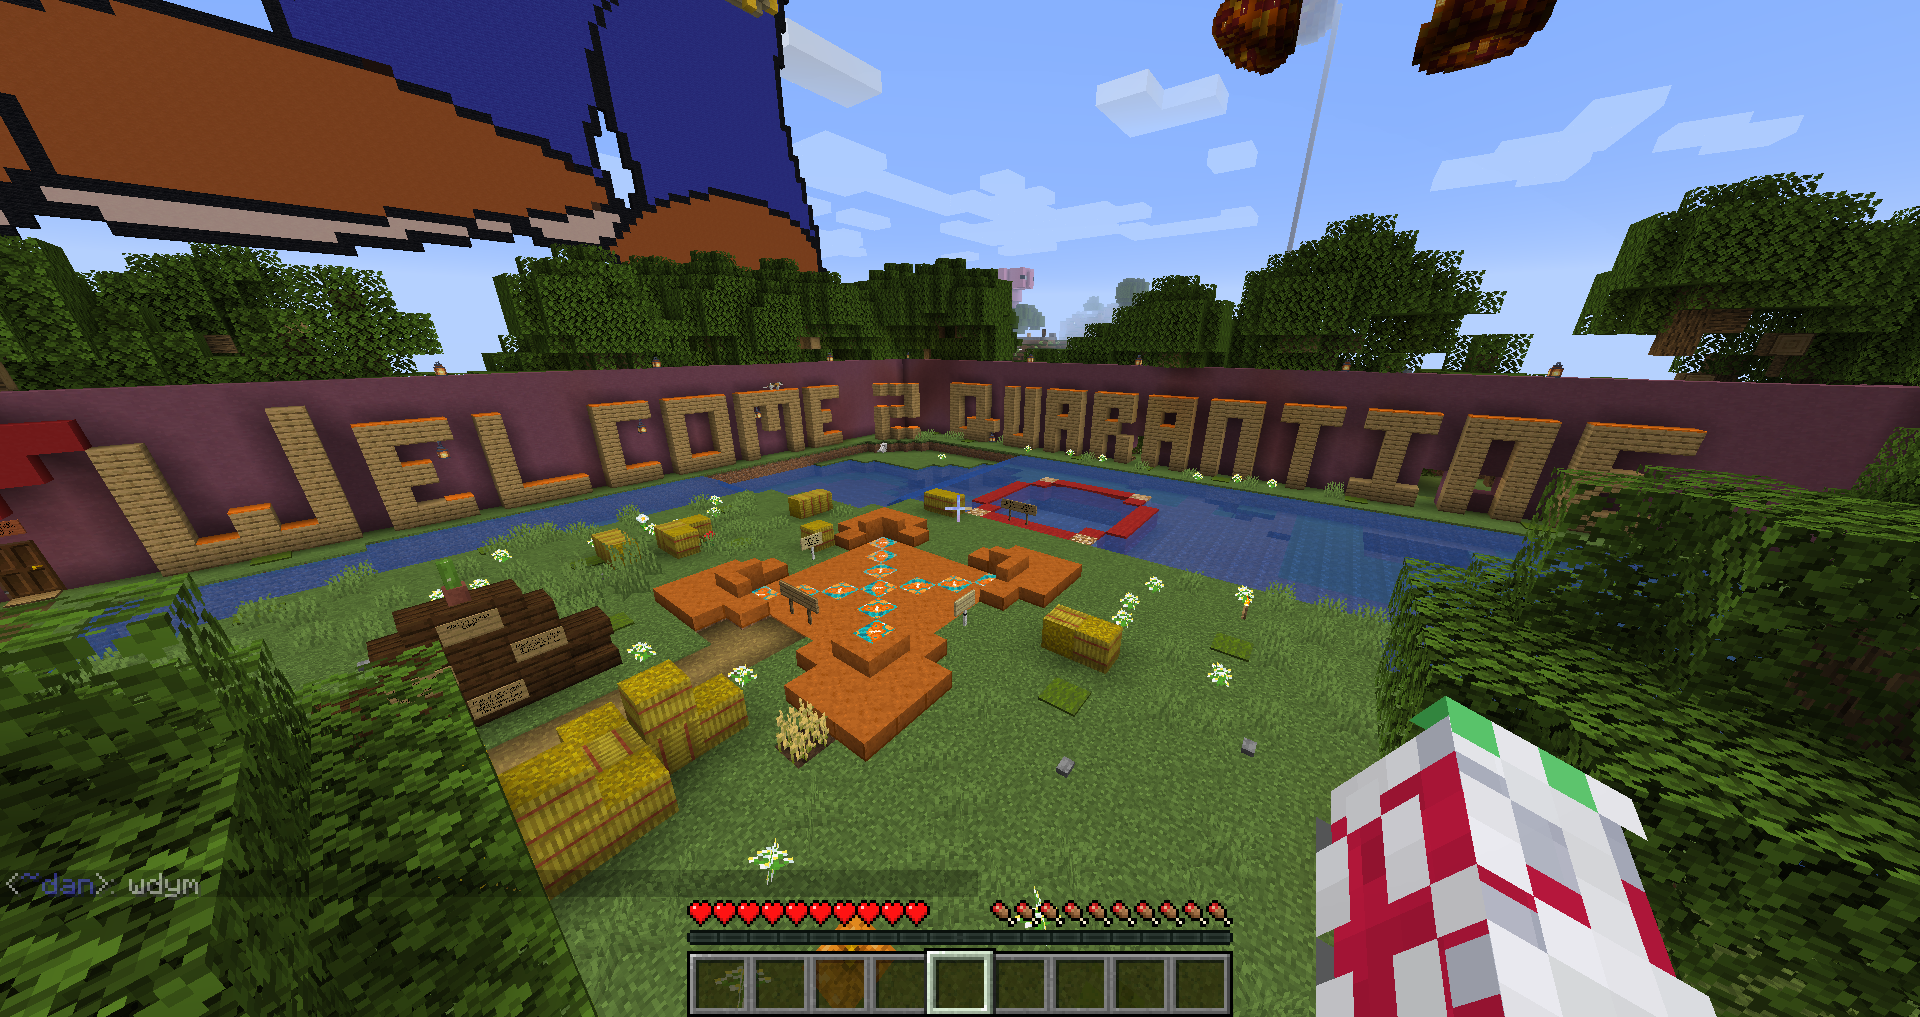
\includegraphics[width=\textwidth]{screenshot_2020-04-18_91.121.134.152.png}
	\caption{The welcome area to a server in France entitled \enquote{Coronavirus Quarantine.}}
	\label{fig:spawnsign}
\end{figure}

\begin{figure}[t]
	\centering
	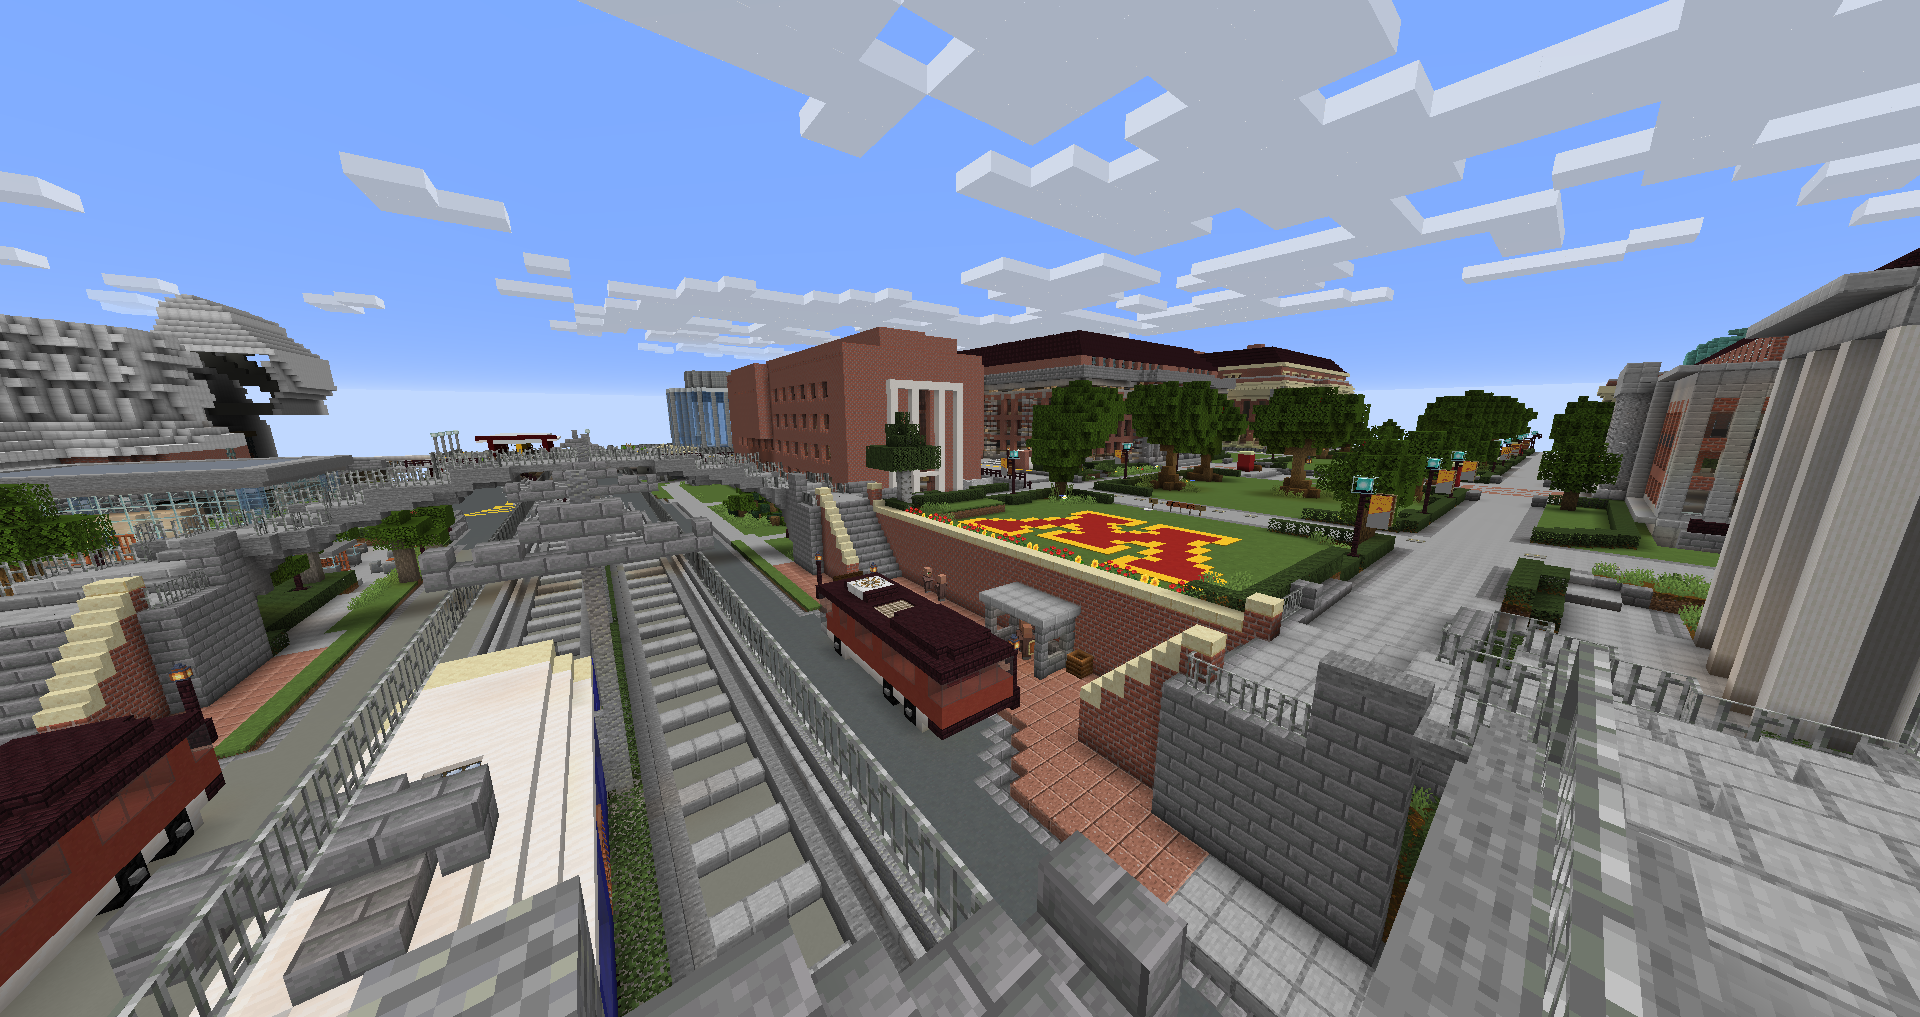
\includegraphics[width=\textwidth]{screenshot_2020-04-25_goldycraft.png}
	\caption{Looking Northwest from a bridge over the light rail line on a \mc\ server dedicated to
			reproduction of the University of Minnesota Twin-Cities campus.}
	\label{fig:goldycraft}
\end{figure}

One aspect of the social structure of these servers that is far less likely to
run afoul of research ethics in its analysis is the built environment. On one server,
the welcome area consisted of an enormous sign reading
\enquote{WELCOME 2 QUARANTINE}~(Fig.~\ref{fig:spawnsign}), indicating a dedication of
the game to the idea of a quarantine escape beyond simply a comedic \ac{motd}.

Another form of construction is the recreation of a real environment no longer
accessible during quarantine.
As college students are forced to flee home, many experience a
homesickness in the loss of their familiar campuses. Thanks to a semester spent
in a University of Minnesota program, I have found myself in a Facebook group
entitled \enquote{UMN Memes for Frozen Northern Teens,} which satirizes life
on the campus. As quarantine escalated, I saw calls for assistance in constructing
a faithful reproduction of the entire university campus. This server experienced a rapid
increase in membership, and is now effectively a virtual clone of the university (Fig.~\ref{fig:goldycraft}).

This was not limited to Minnesotans, as was noted by \textcite{Anderson2020} in a
blog post surveying several concurrent projects in universities as disparate as South Louisiana
Community College and Boston University. Far from escapism, the use of online \mc\ servers
permits a counterintuitive return to the real world: an experience of one's own
environment both idealized in its unchaging pristine state, locked at high noon and 
subject to the will of whomever controls the server; yet simultaneously flawed
in that it remains only an approximation bound to the
\enquote{rules that operate in the universe constructed by the game}~\parencite[222]{Manovich2001},
in this case a finite material selection restricted to \SI{1}{\cubic\metre} cubes.

\subsection{Tabletop Games}

Board games play an integral role in human culture, with evidence of their
existence apparent for millenia in areas as disparate as Mesoamerica~\parencite{Voorhies2013}
and Southern Africa~\parencite{Townshend1979}. During a period of social distancing,
this specific form of social interaction is impossible as people are physically isolated.
The video game \tbl~\parencite{Tabletop} however allows a simulation of the board game
experience. By simply being a physics engine connected to a multiplayer network, players
can use a computer to play effectively any board or card game as if they were around
a table in real life. Throughout the \ac{covid} crisis, I have had the opportunity to
play a wide variety of card games with friends using this technology, which has been
enjoyable. However, the experience is by no means equivalent to playing in real life.

The initial hurdle in using \tbl\ is in mastering the controls. When in real life drawing
an extra card from a stack could be easily corrected by placing it back on top using one's
non-dominant hand or an expert manipulation of one's fingers, it becomes a hassle when
limited to a mouse pointer. It is easy to misplace or mismaneuver items on the table,
causing the game to slow down in a way one would never see in a real life game.

The more salient difference -- and what I consider to be more anthropologically
intriguing -- between the experiences of real-life tabletop gameplay and that of
\tbl\ is the lack of human connection. While I have always played the games with
some audio chat running to allow talking to my friends, playing \tbl\ has
allowed me to discover how much gesture and facial expressions mediate communication
in the setting of a tabletop game. In a game of poker, for instance, it becomes exceptionally
difficult to tell if an opponent is bluffing: without facial expressions all a player can
use is their voice, and an unreliable source of voice at that. Players can feign network
problems for going silent rather than attempt to lie if they feel as if their tone
of voice may betray them. Even the most simple mechanic of gameplay -- taking turns -- becomes
a slow and arduous process. While I see no real difference between saying \enquote{okay,
your turn} in real life versus virtually, it somehow becomes more alien and even
confusing within \tbl. I cannot tease out what makes turn-taking so seamless in real
life gameplay, and following the end of quarantine I intend to study gameplay carefully
to see what visual cues accompany play that are absent from \tbl.

\section{Video Chat}

The experience of videoconferencing is not in any sense new to twenty-first century
American life. However, the change from in-person classes to virtual brings with
it a somewhat novel social experience. In one class on paleolithics, it was no
longer possible to fracture rocks in the controlled environment of a classroom.
Instead, we were tasked with going outdoors and finding rocks that looked promising
for the task despite our inexpertise in identifying rock types.
Artifacts had to be displayed via grainy webcam video rather than felt in students'
hands, undoubtedly detracting from a tangible understanding of how fracture
patterns work and indicate technological properties.

In another class, the discussion sections began quarantine with concurrent video
chat, where all two dozen students had video trained on their faces for the
hour-long class. As the semester progressed, fewer and fewer students chose to
enable video, preferring to only communicate via audio. I actually had a hard
drive failure on my laptop mid-quarantine
and had to move to a desktop with no webcam, thus ending any ability to join
video chat for the rest of the semester.
In the final discussion section of this class, not a single student had their
video enabled. This occurred without any explicit discussion of the rules regarding
discussion participation; rather, students collectively decided not to show their
faces and seemingly overwhelmed the TA to the point it became the norm.
The students' ability to control the structure and social setting of a class would
be shocking if it occurred in an in-person setting, yet when over Zoom it was 
effortlessly accepted.

\section{Contact Tracing and the Future of the Personal Smartphone}

In an epidemic, some degree of trust in authority is required of the
public at large. Doctors, for example, are the sole holders of the
requisite training to diagnose and treat patients. Public health officials
are understood to likewise have knowledge in disease prevention, and are
thus entrusted with the ability to advise and dictate behavior. This
conscious choice to entrust the powerful with greater authority during an
emergency is neither novel nor concerning in and of itself, but the use of tecnhology in
the \ac{covid} crisis and its aftermath is interesting in its potential to
affect social and power relations.

\subsection{Surveillance}

In attempting to inhibit the transmission of \ac{virus}, scientists and public
agencies have explored the viability of the use of surveillance technologies.
\textcite{Ferretti2020} argue that manual contact tracing methods thus far employed
(interviews with patients, individual isolation) are insufficient at halting the
spread of disease. They explicitly call for a technological solution as the only
effective method of disease prevention, specifically via smartphone tracking.

In China, where \ac{virus} was first identified, the initial stages of smartphone
surveillance were implemented. In order to access public transportation and some
other services outside the home, citizens were required to use a smartphone app
which opaquely identified themselves as permitted or prohibited from the service
they attempted to access~\parencite{NYT.alipay}.
Studying public response to the SARS outbreak at the turn of the twenty-first century,
\textcite{Lee2009} note that public health crises often cause the public
to pay great attention to and critique the bureaucratic nature of the state.
The state's ability to control movement, from blocking access to the subway to
changing the date of the New Year~\parencite{Chen2020}, is far more easily percieved
under these crisis situations.

\subsection{Contact Tracing}

Scholars of computer science and mathematics have worked toward some method of
performing the contact tracing outlined by \textcite{Ferretti2020}. The most
prominent of these is currently \ac{dp3t}, an evolving suite of algorithms
under development in Europe by \textcite{DP-3T}. The main methodology of
\ac{dp3t} is the continuous transmission and reception of emphemeral identifiers
by all enabled devices, such that every device in the system would possess a log
of every device which it had encountered in the past. When a person is declared
infected, the ephemeral signals transmitted over the course of their
infectious period would be publicised, allowing every device which had
encountered the infected person's phone to notify its user of potential exposure.
The \ac{dp3t} designers have gone to great lengths to design a fully-anonymous
system without location data or tracking potential, and their cryptographic work
is commendable. However, the authors' original release of the proposal was
explicitly just that -- a proposal: \enquote{we are publishing this document to
seek feedback from a broad audience on the high-level design, its security and
privacy \dots\ so that further protection mechanisms can be added}~\parencite[2]{DP-3T}.

Despite these qualms, \textcite{AppleCT.Announcement} announced a collaborative
derivative project to introduce this form of contact tracing to millions of
smartphones. Along with releasing documentation for software developers at public
health institutions to implement the system~\parencite*{AppleCT.API}, they have also
published information on how the Bluetooth~\parencite*{AppleCT.Bluetooth} and
crypotography~\parencite*{AppleCT.Crypto} are expected to operate.
While the latter two documents include statements on privacy protection, they lack
the discussion of protections against state-level adversaries that make up
much of the \ac{dp3t} proposal.
Regardless, it is expected that by the end of the year, devices manufactured by
\citeauthor{AppleCT.Announcement} will be constantly broadcasting and listening
for these contact signals. If the \ac{covid} crisis persists by the time this
becomes an integral part of smartphone operating systems, it will likely be the
norm for people to experience notifications warning them of previous contact
with an infectious person.

While the privacy implications of broadcasting one's presence are of course 
wide-reaching, I am intrigued by what this will mean for our personal relations
to our devices. The implication made by both the cryptographic research team
and the corporate manufacturers is that our devices are extensions of our bodies.
Our expulsion of viral particles emanating from our respiration, an exclusively physical and biological act,
is in the minds of the proposals inexorably tied to the virtual signals of our
smartphones emanating from our pockets. 
Every physical interaction between people, no matter how brief, will be logged.
So long as both participants have up-to-date smartphones, they will exchange
information. While phone notifications of potential infection persist, people
will become more and more aware of this logging and transmission, further
entrenching the idea of the phone as a part of the body.

\subsection{Access and Cross-Cultural Considerations}

Not everyone has a smartphone. In fact, it is likely that smartphone owners
constitute a minority of the global population~\parencite{pew.phone}.
People's lack of smartphones can occur for socioeconomic, political, or
reasons of personal choice. Should
smartphones become a major part of public health diagnosis and communication,
those most likely to possess them (the young, the educated, and the rich) will
have greater access to warnings regarding illness. 
Those without still have biological bodies capable of transmitting and receiving
illness, but without the technological appendage capable of transmitting and
receiving signals, they are excluded from perceptions of epidemic transmission.

Conceptions of privacy differ amongst societies. The implementation of a
sudden and global change to smartphones could cause rifts between people and
between societies. The conception of privacy in Islamic societies, as detailed
by \textcite{Abokhodair2016}, for instance, may be alien to the software
developers in California who are implementing the contact tracing systems.

The moment the first batch of notifications appear on smartphones reading
\enquote{you have been near someone infected with \ac{covid} in the last
fourteen days} I believe will be a moment that both the individual recipients
and global society as a whole find unforgettable. The relation of technology to the
body will not be the same after this crisis.

\printbibliography

\end{document}